\chapter{Procesamiento Visual}
\label{cap:procesamientoVisual}

En los capítulos anteriores se ha presentado una visión general del proyecto, las principales tecnologías utilizadas y los trabajos relacionados más relevantes. A partir de este capítulo comienza la descripción del sistema desarrollado, organizada siguiendo las grandes fases del pipeline.

Este capítulo se centra en la primera parte del sistema: el procesamiento visual del vídeo broadcast. Su objetivo es transformar los frames originales del partido en una representación estructurada de los elementos del juego. Para ello se describen las etapas de detección de jugadores, árbitros, porteros y balón, la identificación de equipos, la estimación geométrica sobre el terreno de juego y el tracking multiobjeto empleado para mantener identidades consistentes a lo largo del vídeo.

La salida de este bloque visual sirve como base para los capítulos posteriores, donde se analizan aspectos futbolísticos de mayor nivel, como la posesión, las posiciones de los jugadores y los eventos del partido, en el \hyperref[fig:arquitectura-software]{Capítulo~\ref*{cap:analisisTactico}} , y finalmente se genera la narración automática en texto y audio, descrita en el \hyperref[cap:narracion]{Capítulo~\ref*{cap:narracion}}.

Antes de entrar en cada etapa, resulta útil tener en mente un frame del vídeo original, es decir, la entrada del sistema antes de aplicar cualquier tipo de procesamiento. La \hyperref[fig:raw-football-image]{Figura~\ref*{fig:raw-football-image}} muestra un ejemplo de frame de entrada utilizado por el pipeline.

\begin{figure}[H]
    \centering
    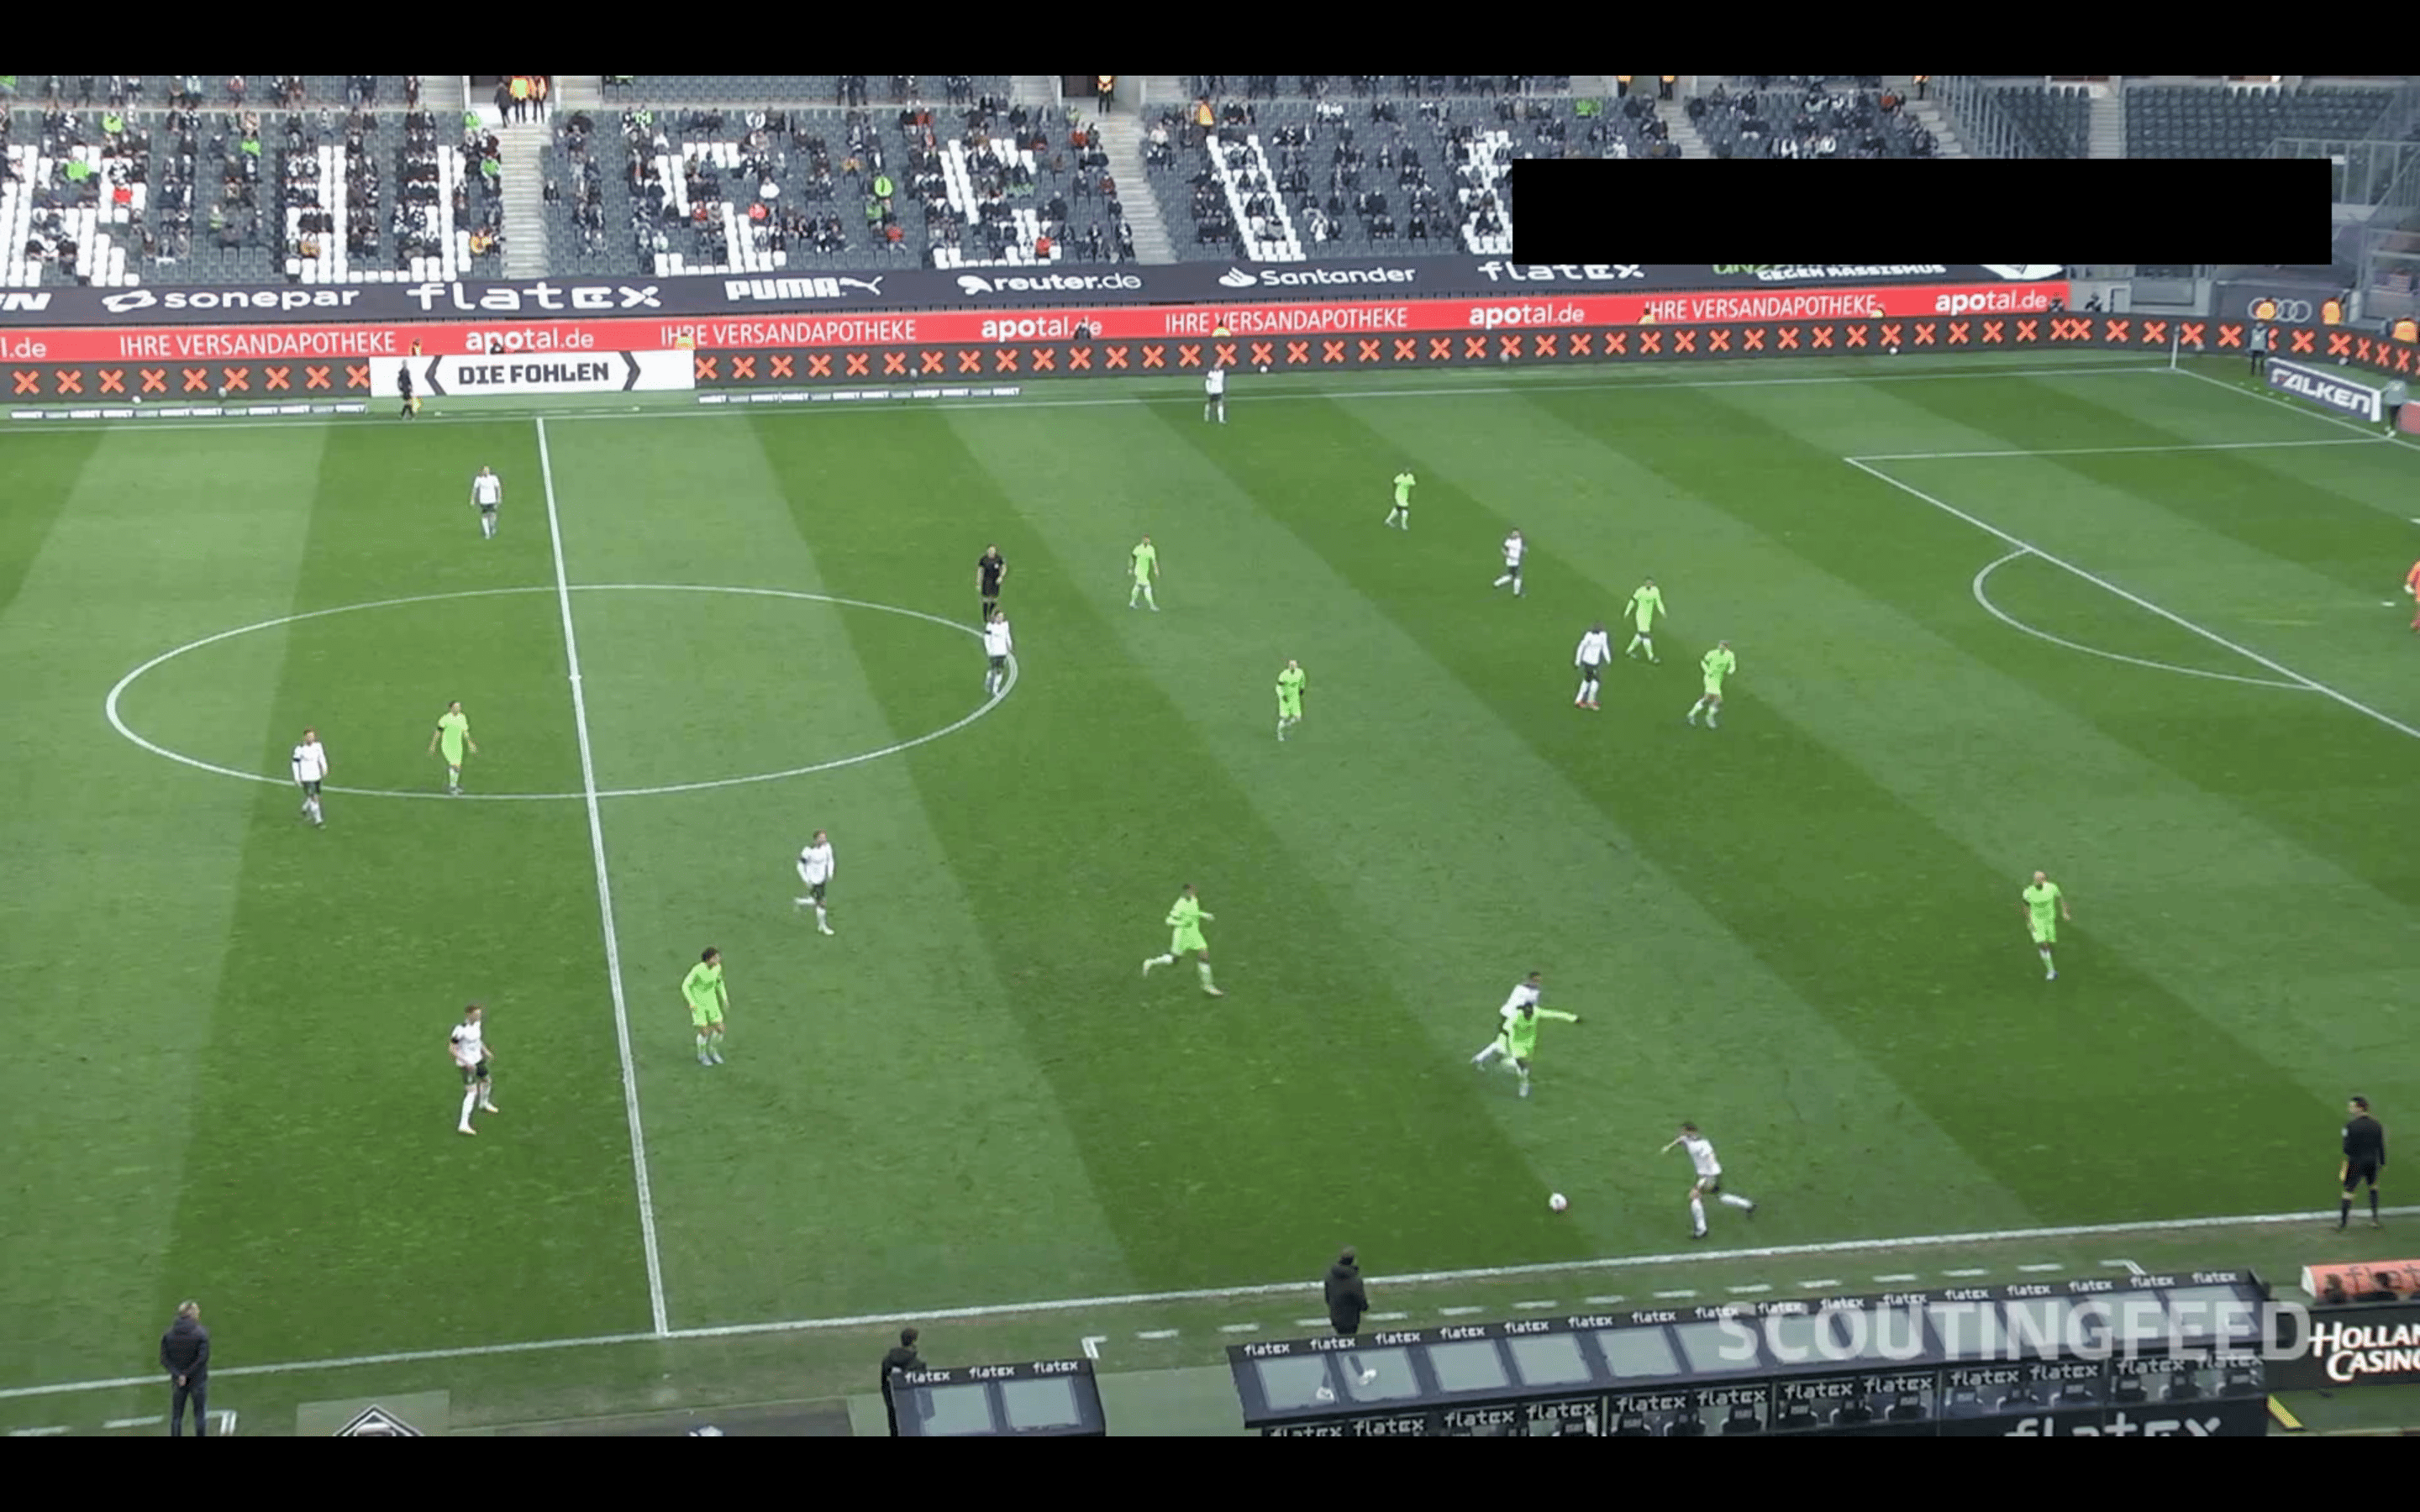
\includegraphics[width=0.9\textwidth]{Imagenes/Propias/Raw_image.png}
    \caption[Frame original del vídeo de entrada]{
    Frame original del vídeo de entrada antes de aplicar detección, calibración, identificación de equipos o tracking.
    }
    \label{fig:raw-football-image}
\end{figure}


\section{Detección de elementos del juego}
\label{sec:deteccion-elementos-juego}

La primera fase del pipeline consiste en detectar, fotograma a fotograma, los elementos relevantes del partido. Para esta tarea se empleó YOLOv11m, donde la letra \texttt{m} hace referencia a la variante \textit{medium}, elegida por ofrecer un compromiso razonable entre precisión y coste computacional.

Como punto de partida se utilizó el modelo base, es decir, el modelo preentrenado sin adaptación específica al dominio futbolístico. Al aplicarlo directamente sobre vídeo de fútbol, el modelo detecta jugadores, árbitros y porteros principalmente como instancias de la clase \texttt{person}, mientras que el balón puede aparecer como \texttt{sports ball}. Esto puede observarse en la \hyperref[fig:raw-detection-yolo11m]{Figura~\ref*{fig:raw-detection-yolo11m}}. Esta salida inicial permite comprobar que el detector reconoce objetos relevantes en la escena, pero no proporciona todavía la separación semántica necesaria para el proyecto, ya que agrupa todos los participantes humanos en una misma clase.

\begin{figure}[H]
    \centering
    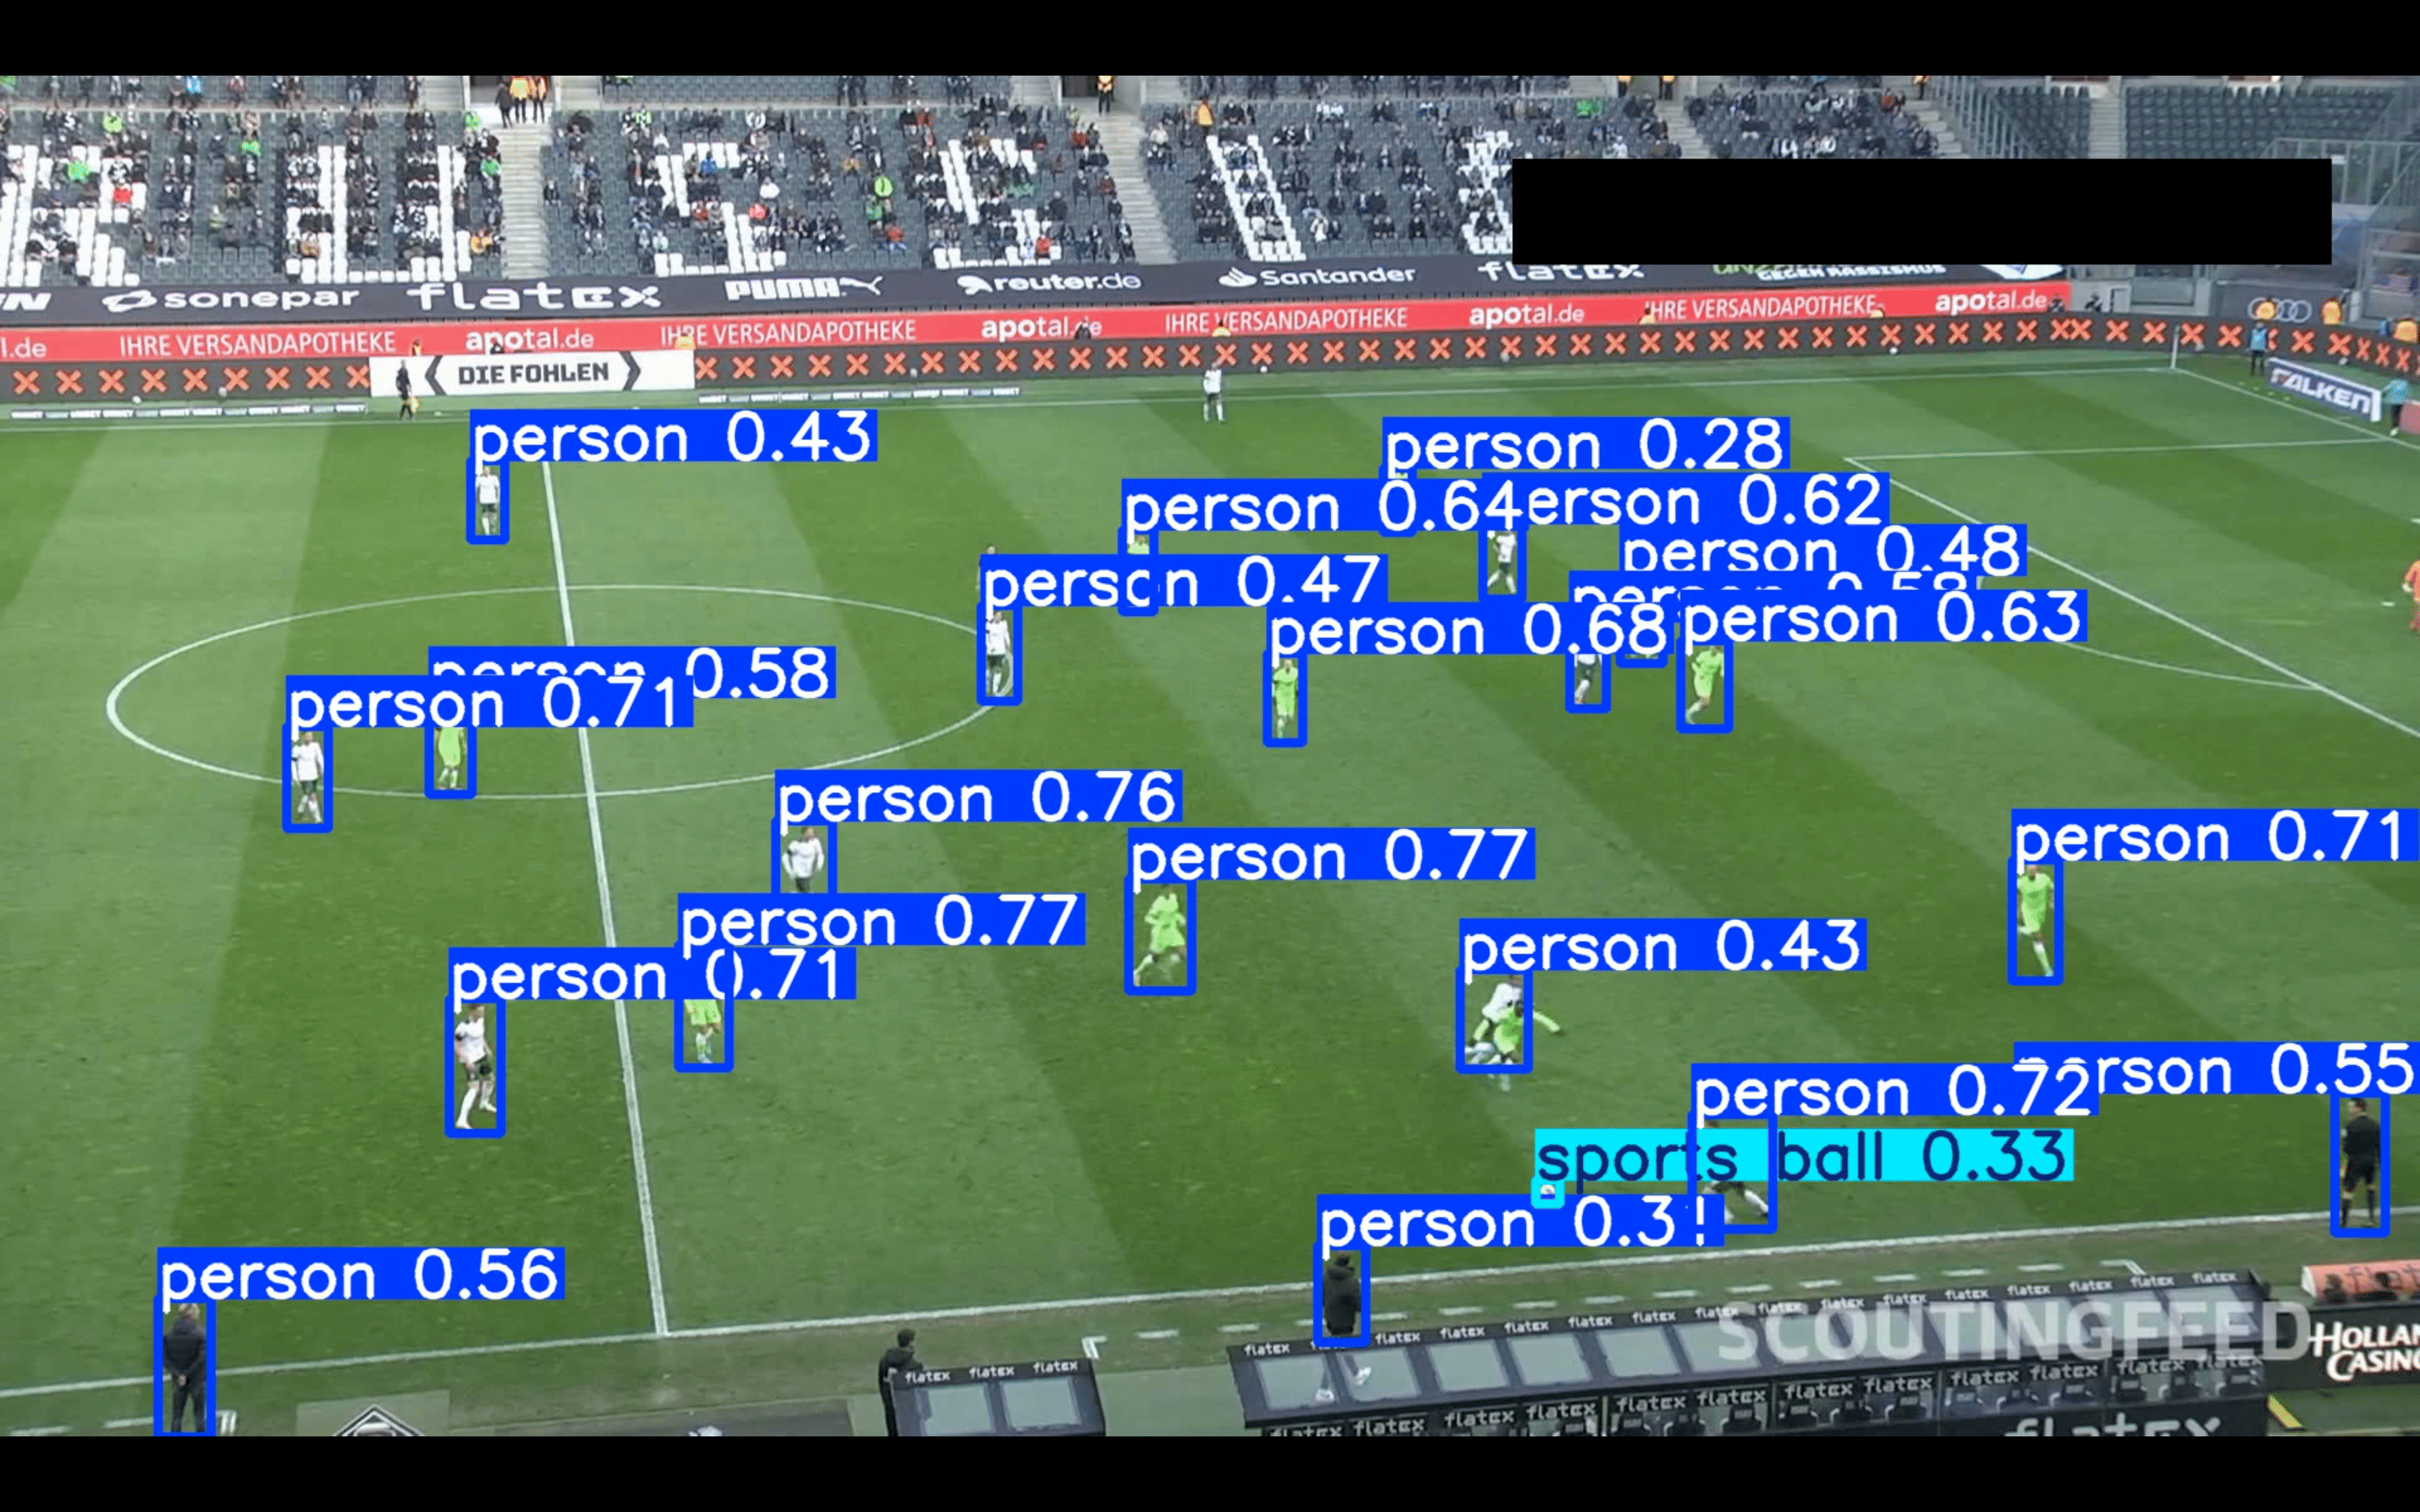
\includegraphics[width=0.9\linewidth]{Imagenes/Propias/Raw_detection.png}
    \caption[Detección inicial con YOLOv11m]{Detección inicial realizada con YOLOv11m base sobre un frame del partido.}
    \label{fig:raw-detection-yolo11m}
\end{figure}

Para observar el comportamiento del modelo base se realizó una prueba exploratoria sobre un clip corto de 10 frames. YOLO proporciona para cada detección un valor de confianza (\textit{confidence}), que representa la seguridad estimada del modelo respecto a la clase predicha. Los resultados se muestran en la Tabla \ref{tab:yolo11mBaseFrame}.

\begin{table}[H]
	\centering
	\begin{tabular}{c|c|c|c|c}
		\textbf{Frame} & \textbf{Personas} & \textbf{Balón} & \textbf{Conf. media} & \textbf{Conf. max} \\
		\hline\hline
		1 & 22 & 0 & 0.5646 & 0.7637 \\
		2 & 22 & 0 & 0.5741 & 0.7864 \\
		3 & 22 & 0 & 0.5724 & 0.7894 \\
		4 & 23 & 1 & 0.5370 & 0.7900 \\
		5 & 23 & 1 & 0.5094 & 0.7775 \\
		6 & 23 & 0 & 0.5514 & 0.7846 \\
		7 & 23 & 0 & 0.5571 & 0.7727 \\
		8 & 21 & 1 & 0.5781 & 0.7730 \\
		9 & 20 & 1 & 0.6162 & 0.7941 \\
		10 & 19 & 1 & 0.5925 & 0.7862 \\
		\hline
	\end{tabular}
	\caption[Prueba exploratoria de detección con YOLOv11m]{Prueba exploratoria de detección con YOLOv11m base sobre un clip corto de 10 frames.}
	\label{tab:yolo11mBaseFrame}
\end{table}

Los resultados muestran que el modelo detecta de forma estable a las personas presentes en la escena, con entre 19 y 23 detecciones por frame. Sin embargo, la detección del balón resulta más irregular, ya que solo aparece en 5 de los 10 frames analizados.

Sin embargo, para este proyecto no basta con detectar personas genéricas: es necesario distinguir entre elementos futbolísticos concretos, como jugadores, árbitros, porteros y balón. Por este motivo se decidió adaptar el detector mediante \textit{fine-tuning}.

\subsection{Adaptación del detector mediante \textit{fine-tuning}}
Como el modelo YOLOv11m base no proporcionaba la separación semántica necesaria para el proyecto, se decidió adaptar el detector al dominio futbolístico mediante \textit{fine-tuning}. El objetivo era que el modelo no solo detectara personas genéricas, sino que distinguiera entre clases relevantes para el sistema, como jugadores, árbitros, porteros y balón.


\subsubsection{Conjuntos de datos utilizados}

Para esta adaptación se emplearon tres conjuntos de datos con funciones distintas dentro del proceso de entrenamiento. La \hyperref[tab:datasets-finetuning-yolo]{Tabla~\ref*{tab:datasets-finetuning-yolo}} resume su procedencia, clases anotadas, tamaño y uso dentro del proyecto.

\begin{table}[H]
\centering
\scriptsize
\renewcommand{\arraystretch}{1.25}
\begin{tabularx}{\textwidth}{
>{\raggedright\arraybackslash}p{2.4cm}
>{\raggedright\arraybackslash}X
>{\raggedright\arraybackslash}p{2.8cm}
>{\raggedright\arraybackslash}p{2.5cm}
>{\raggedright\arraybackslash}X
}
\toprule
\textbf{Dataset} & \textbf{Url} & \textbf{Clases} & \textbf{Tamaño / partición} & \textbf{Uso} \\
\midrule

Roboflow fútbol \label{} &
\href{https://universe.roboflow.com/yolo-atnlh/football-detection-wfhdh}{Roboflow - FootBall Detection Computer Vision Model} &
\texttt{ball}, \texttt{player}, \texttt{referee}, \texttt{goalkeeper} $\rightarrow$ \texttt{player}. &
Train/val/test: 612/38/13 &
Primer \textit{fine-tuning} supervisado con clases futbolísticas. \\

\midrule

Datos sintéticos &
\href{https://research.spiideo.com/login/main.html}{Spiideo SoccerNet SynLoc} &
\texttt{person} $\rightarrow$ \texttt{player}. &
Train/val/test: 42.554/6.777/9.309 &
Adaptación intermedia sintética al dominio futbolístico: césped, jugadores, variación de cámara, iluminación y desenfoque de movimiento.. \\

\midrule

DFL-Bundesliga &
\href{https://universe.roboflow.com/inkyu-sa-e0c78/dfl-bundesliga-soccer-football-gpqdy}{Roboflow - DFL-Bundesliga} &
\texttt{ball}, \texttt{player}, \texttt{referee}. &
Train/val/test: 19.068/2.434/2.455 &
Refinamiento final sobre datos reales más próximos al escenario objetivo. \\

\bottomrule
\end{tabularx}
\caption[Conjuntos de datos utilizados para el fine-tuning del detector]{
Conjuntos de datos utilizados durante la adaptación del detector YOLOv11m al dominio futbolístico.
}
\label{tab:datasets-finetuning-yolo}
\end{table}

\noindent\textit{Nota:} Para homogeneizar el entrenamiento entre fases, las clases se adaptaron al formato final del detector: \texttt{player}, \texttt{referee} y \texttt{ball}. En SoccerSynth-Detection, la clase original \texttt{person} se mapeó a \texttt{player}; las clases \texttt{referee} y \texttt{ball} se incluyeron en la definición de clases, aunque no tenían instancias anotadas en ese conjunto. En el dataset Roboflow fútbol, la clase \texttt{goalkeeper} se integró dentro de \texttt{player}.

\subsubsection{Estrategias de entrenamiento}

Se exploraron dos estrategias principales de adaptación. La primera consistió en entrenar YOLOv11m directamente sobre el pequeño dataset \textit{Roboflow fútbol} obtenido en Roboflow. Este dataset permitía introducir clases futbolísticas concretas, como \texttt{ball}, \texttt{player}, \texttt{referee} y \texttt{goalkeeper}, y servía como primer intento de especialización del modelo base. Además, el proyecto de Roboflow incluía un modelo de referencia con métricas publicadas de \textit{mAP@50} del 82.1\%, precisión del 96.7\% y recall del 75.2\%. Estas métricas no se interpretan como resultados propios ni como una evaluación del dataset, sino como un indicio inicial de que las anotaciones y la definición de clases podían ser útiles para adaptar el detector al dominio futbolístico.

La segunda estrategia consistió en un \textit{fine-tuning} secuencial. En primer lugar, el modelo se entrenó sobre SoccerSynth-Detection \citep{SoccerSynthDetection2025}, un conjunto sintético orientado a detección en fútbol. Esta fase tenía como objetivo adaptar el detector al dominio visual del fútbol, exponiéndolo a escenas con césped, jugadores, variaciones de cámara, iluminación y desenfoque de movimiento. Posteriormente, el modelo resultante se refinó sobre DFL-Bundesliga, un conjunto de imágenes reales con clases más próximas al problema final: \texttt{ball}, \texttt{player} y \texttt{referee}.

La motivación de esta estrategia secuencial era aprovechar primero la variabilidad controlada de los datos sintéticos y, después, ajustar el modelo sobre datos reales más cercanos al escenario de aplicación. De esta forma, se buscaba mejorar la capacidad de generalización del detector antes de integrarlo en el pipeline completo.

\subsubsection{Resultados del \textit{fine-tuning} secuencial} 

La \hyperref[fig:results_finetuning_compare]{Figura~\ref*{fig:results_finetuning_compare}} muestra las curvas de entrenamiento de las dos fases del \textit{fine-tuning} secuencial. En la fase sintética, las métricas convergen rápidamente y se estabilizan hacia la mitad del entrenamiento, alcanzando un mAP@50-95 final cercano a 0.80. En la fase DFL-Bundesliga, la mejora es más gradual y las métricas finales son menores, con un mAP@50-95 cercano a 0.63.

\begin{figure}[H]
\centering

\begin{minipage}{0.95\textwidth}
    \centering
    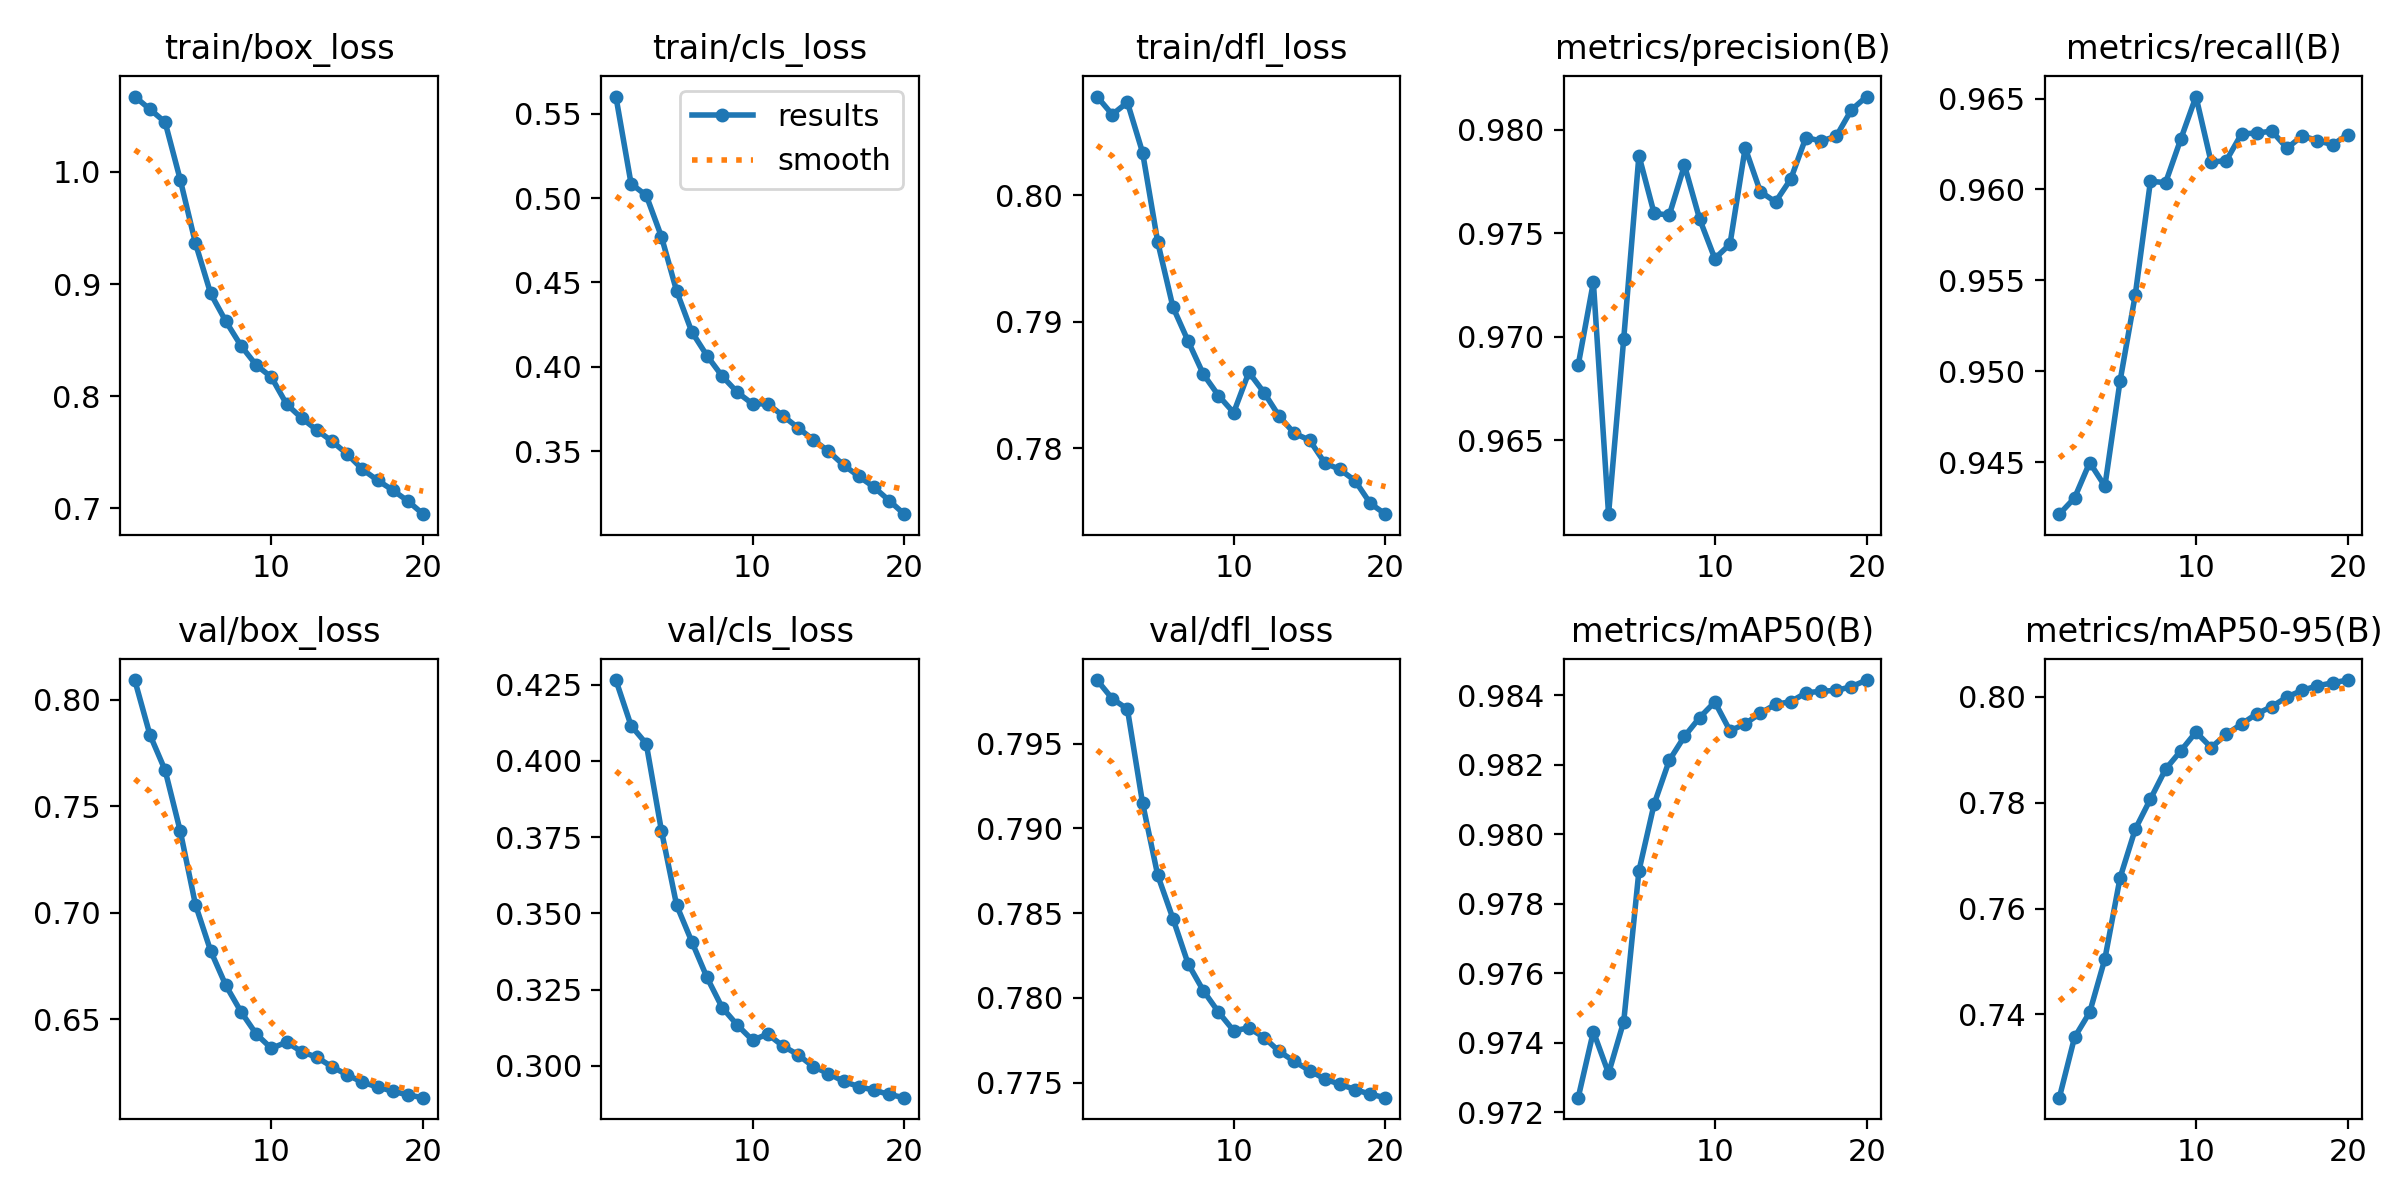
\includegraphics[width=\textwidth]{Imagenes/Propias/results_sinteticos.png}
    \small \textbf{(a)} Primera fase del \textit{fine-tuning} secuencial sobre SoccerSynth-Detection.
\end{minipage}

\vspace{0.4cm}

\begin{minipage}{0.95\textwidth}
    \centering
    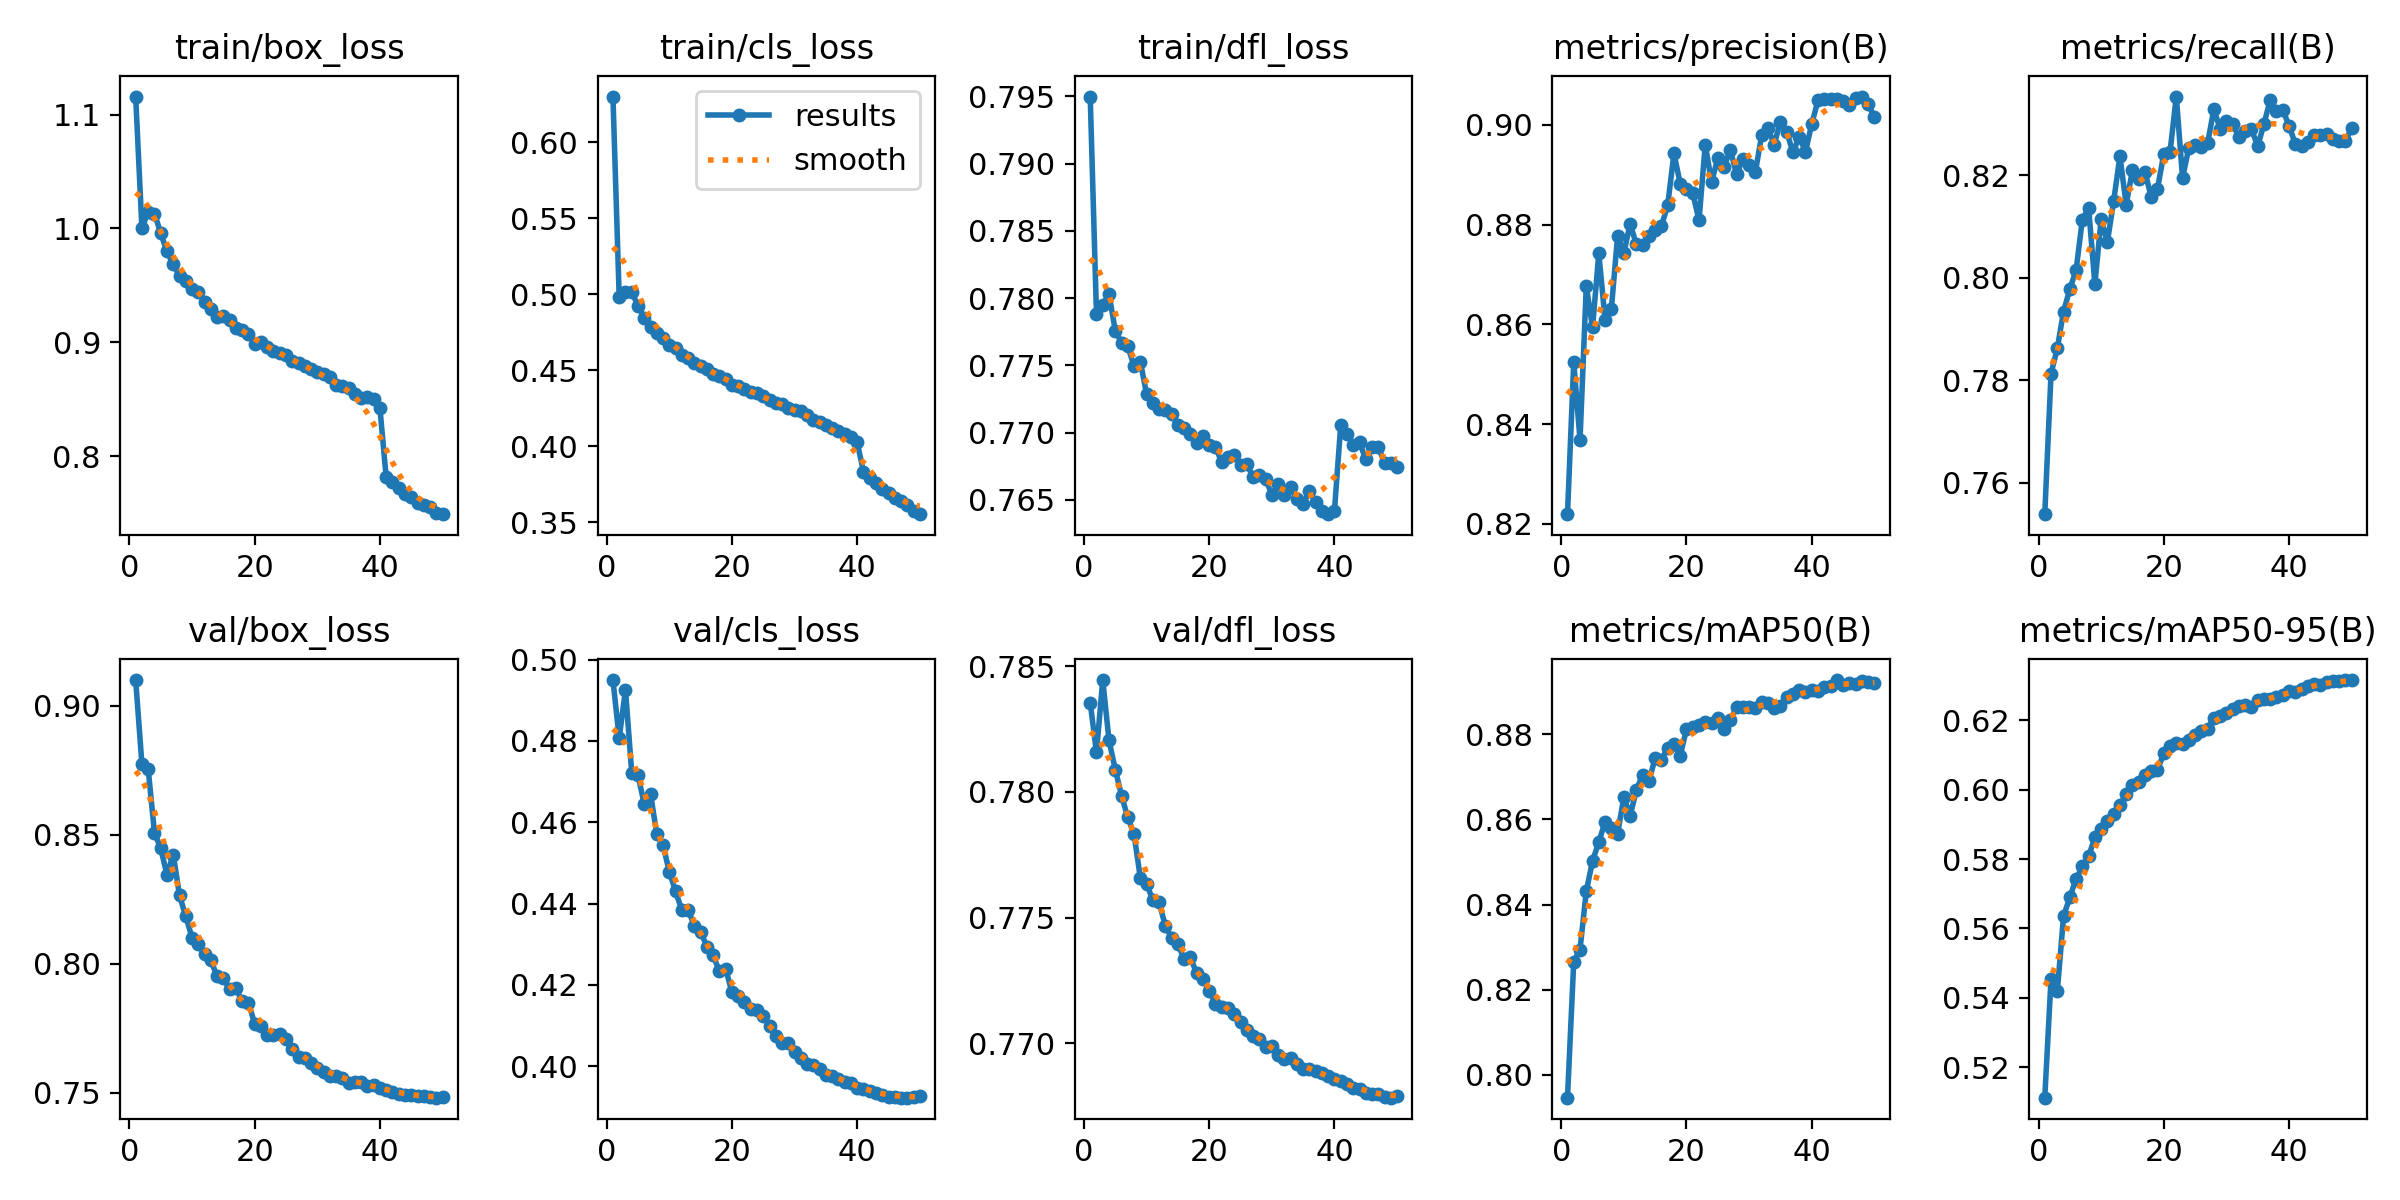
\includegraphics[width=\textwidth]{Imagenes/Propias/results_dfl.png}
    \small \textbf{(b)} Segunda fase del \textit{fine-tuning} secuencial sobre DFL-Bundesliga.
\end{minipage}

\caption[Curvas de entrenamiento del fine-tuning secuencial]{
Curvas de entrenamiento del proceso de \textit{fine-tuning} secuencial.
}
\label{fig:results_finetuning_compare}
\end{figure}

La \hyperref[tab:comparacion_modelos_finetuneados]{Tabla~\ref*{tab:comparacion_modelos_finetuneados}} resume las métricas finales de ambas fases, evaluadas sobre sus respectivos conjuntos de validación. Aunque las métricas de la fase sintética son superiores, no deben interpretarse como una comparación directa entre modelos equivalentes, ya que cada fase utiliza un conjunto de datos distinto. La primera fase sintética trabaja sobre una tarea más simple, homogénea y de una sola clase, mientras que la segunda introduce un dominio más realista y clases más específicas.

\begin{table}[H]
\centering
\scriptsize
\begin{tabular}{c|c|c|c|c|c|c|c}
\textbf{Fase} & \textbf{Ep.} & \textbf{Batch} & \textbf{Imgsz} & \textbf{Prec. final} & \textbf{Recall final} & \textbf{mAP@50} & \textbf{mAP@50-95} \\
\hline\hline
Datos sintéticos & 20 & 8 & 1280 & 0.9816 & 0.9630 & 0.9844 & 0.8032 \\
\hline
DFL-Bundesliga & 50 & 16 & 640 & 0.8911 & 0.8352 & 0.8909 & 0.6305 \\
\hline
\end{tabular}
\caption[Métricas finales del fine-tuning secuencial]{
Métricas finales de validación de las dos fases del \textit{fine-tuning} secuencial.
}
\label{tab:comparacion_modelos_finetuneados}
\end{table}

Para interpretar estas diferencias, la \hyperref[fig:datasets_summary]{Figura~\ref*{fig:datasets_summary}} compara la distribución de clases y las características espaciales de las cajas anotadas en los conjuntos utilizados durante el \textit{fine-tuning} secuencial.

\begin{figure}[H]
\centering

\begin{minipage}{0.55\textwidth}
    \centering
    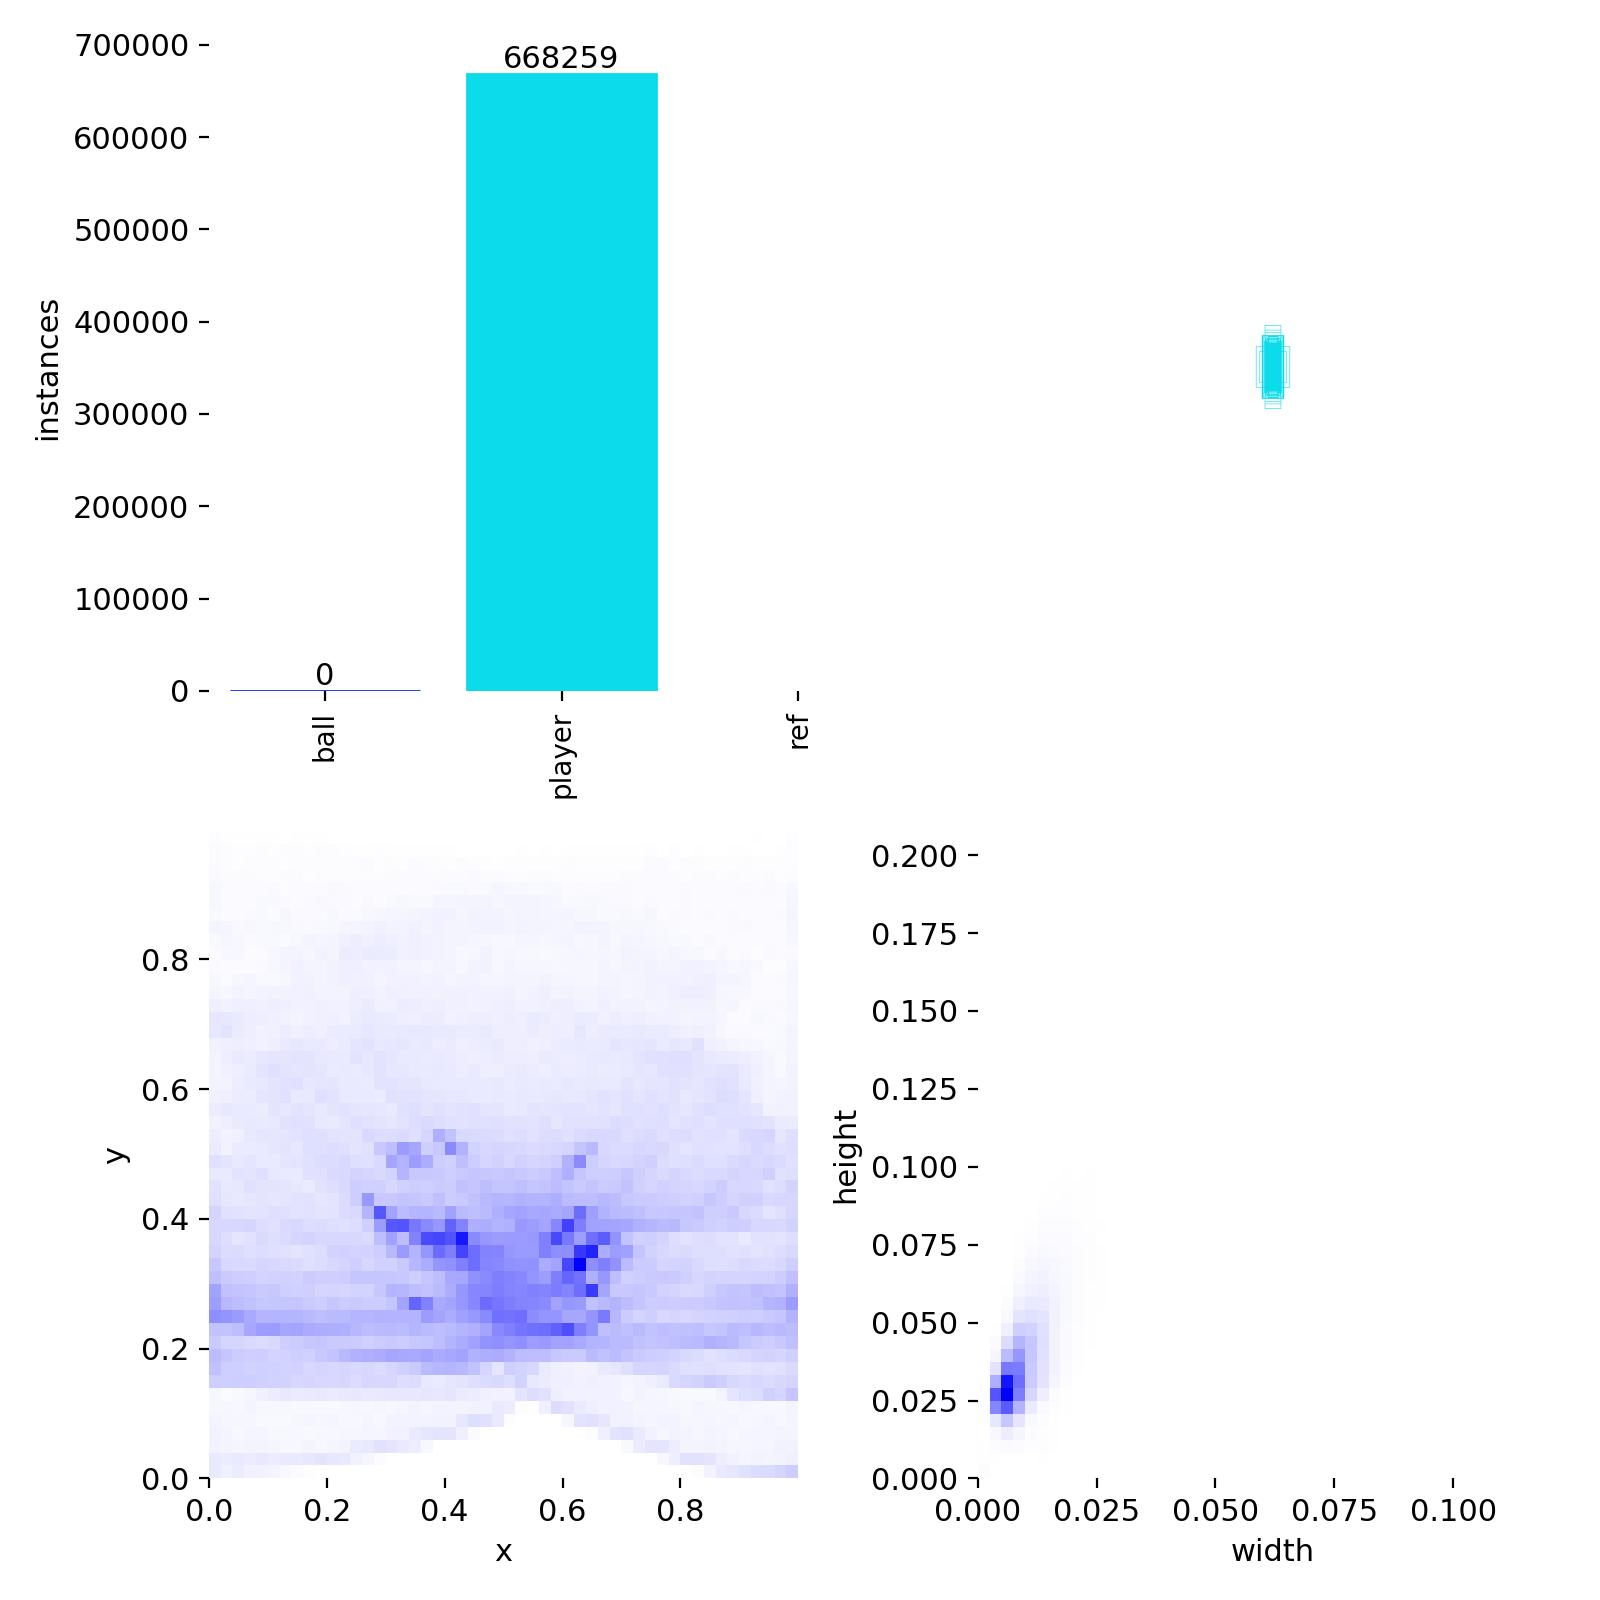
\includegraphics[width=\textwidth]{Imagenes/Propias/labels_sinteticos.jpg}
    \small \textbf{(a)} SoccerSynth-Detection.
\end{minipage}

\vspace{0.4cm}

\begin{minipage}{0.55\textwidth}
    \centering
    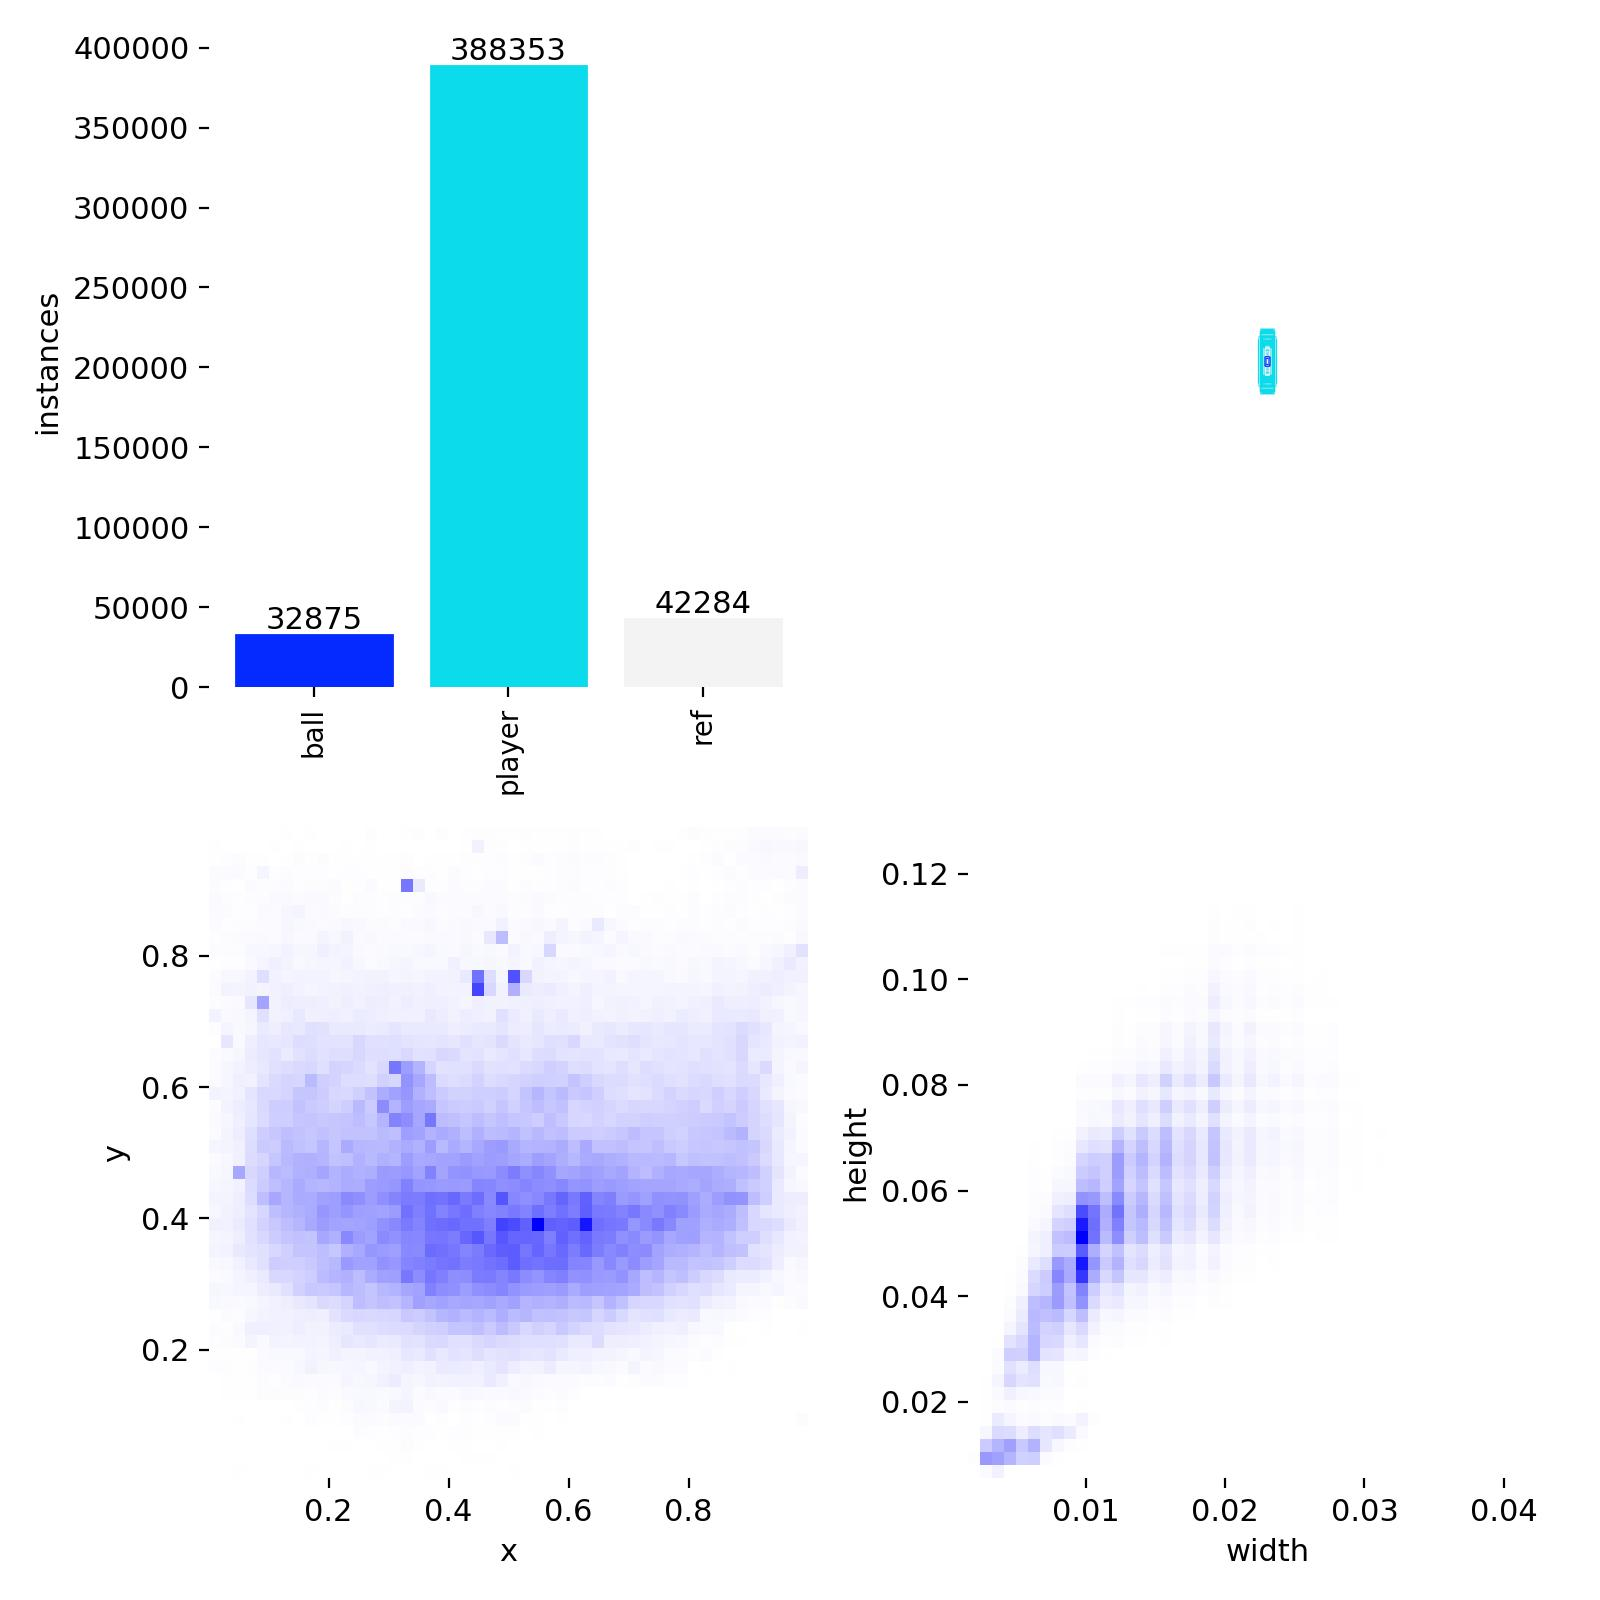
\includegraphics[width=\textwidth]{Imagenes/Propias/labels_dfl.jpg}
    \small \textbf{(b)} Sintéticos + DFL-Bundesliga.
\end{minipage}

\caption[Distribución de etiquetas y cajas en los datasets de fine-tuning]{
Distribución de clases, posiciones normalizadas y tamaños de las cajas delimitadoras en los conjuntos utilizados durante el \textit{fine-tuning} secuencial.
}
\label{fig:datasets_summary}
\end{figure}

Como se aprecia en la \hyperref[fig:datasets_summary]{Figura~\ref*{fig:datasets_summary}}, los datos sintéticos están centrados en la detección de jugadores, mientras que DFL-Bundesliga introduce clases adicionales: balón y árbitro. Por tanto, la segunda fase no solo trabaja sobre imágenes reales, sino también sobre un problema más complejo y desbalanceado. Esto explica que las métricas sean inferiores respecto a la fase sintética sin que ello implique necesariamente un empeoramiento del detector.

La \hyperref[fig:confusion_finetuning_compare]{Figura~\ref*{fig:confusion_finetuning_compare}} muestra las matrices de confusión obtenidas en las dos fases del \textit{fine-tuning} secuencial. En la fase sintética, como ya se había comentado, solo aparece la clase \texttt{player}, con un rendimiento bastante bueno. En la fase DFL-Bundesliga, en cambio, aparecen clases adicionales como \texttt{ball} y \texttt{ref}, lo que permite analizar mejor los errores entre categorías del dominio futbolístico. En particular, se observa que la clase \texttt{player} presenta un comportamiento más estable, mientras que clases menos frecuentes o visualmente más difíciles, como \texttt{ball} y \texttt{ref}, introducen mayor complejidad.

\begin{figure}[H]
\centering

\begin{minipage}{0.55\textwidth}
    \centering
    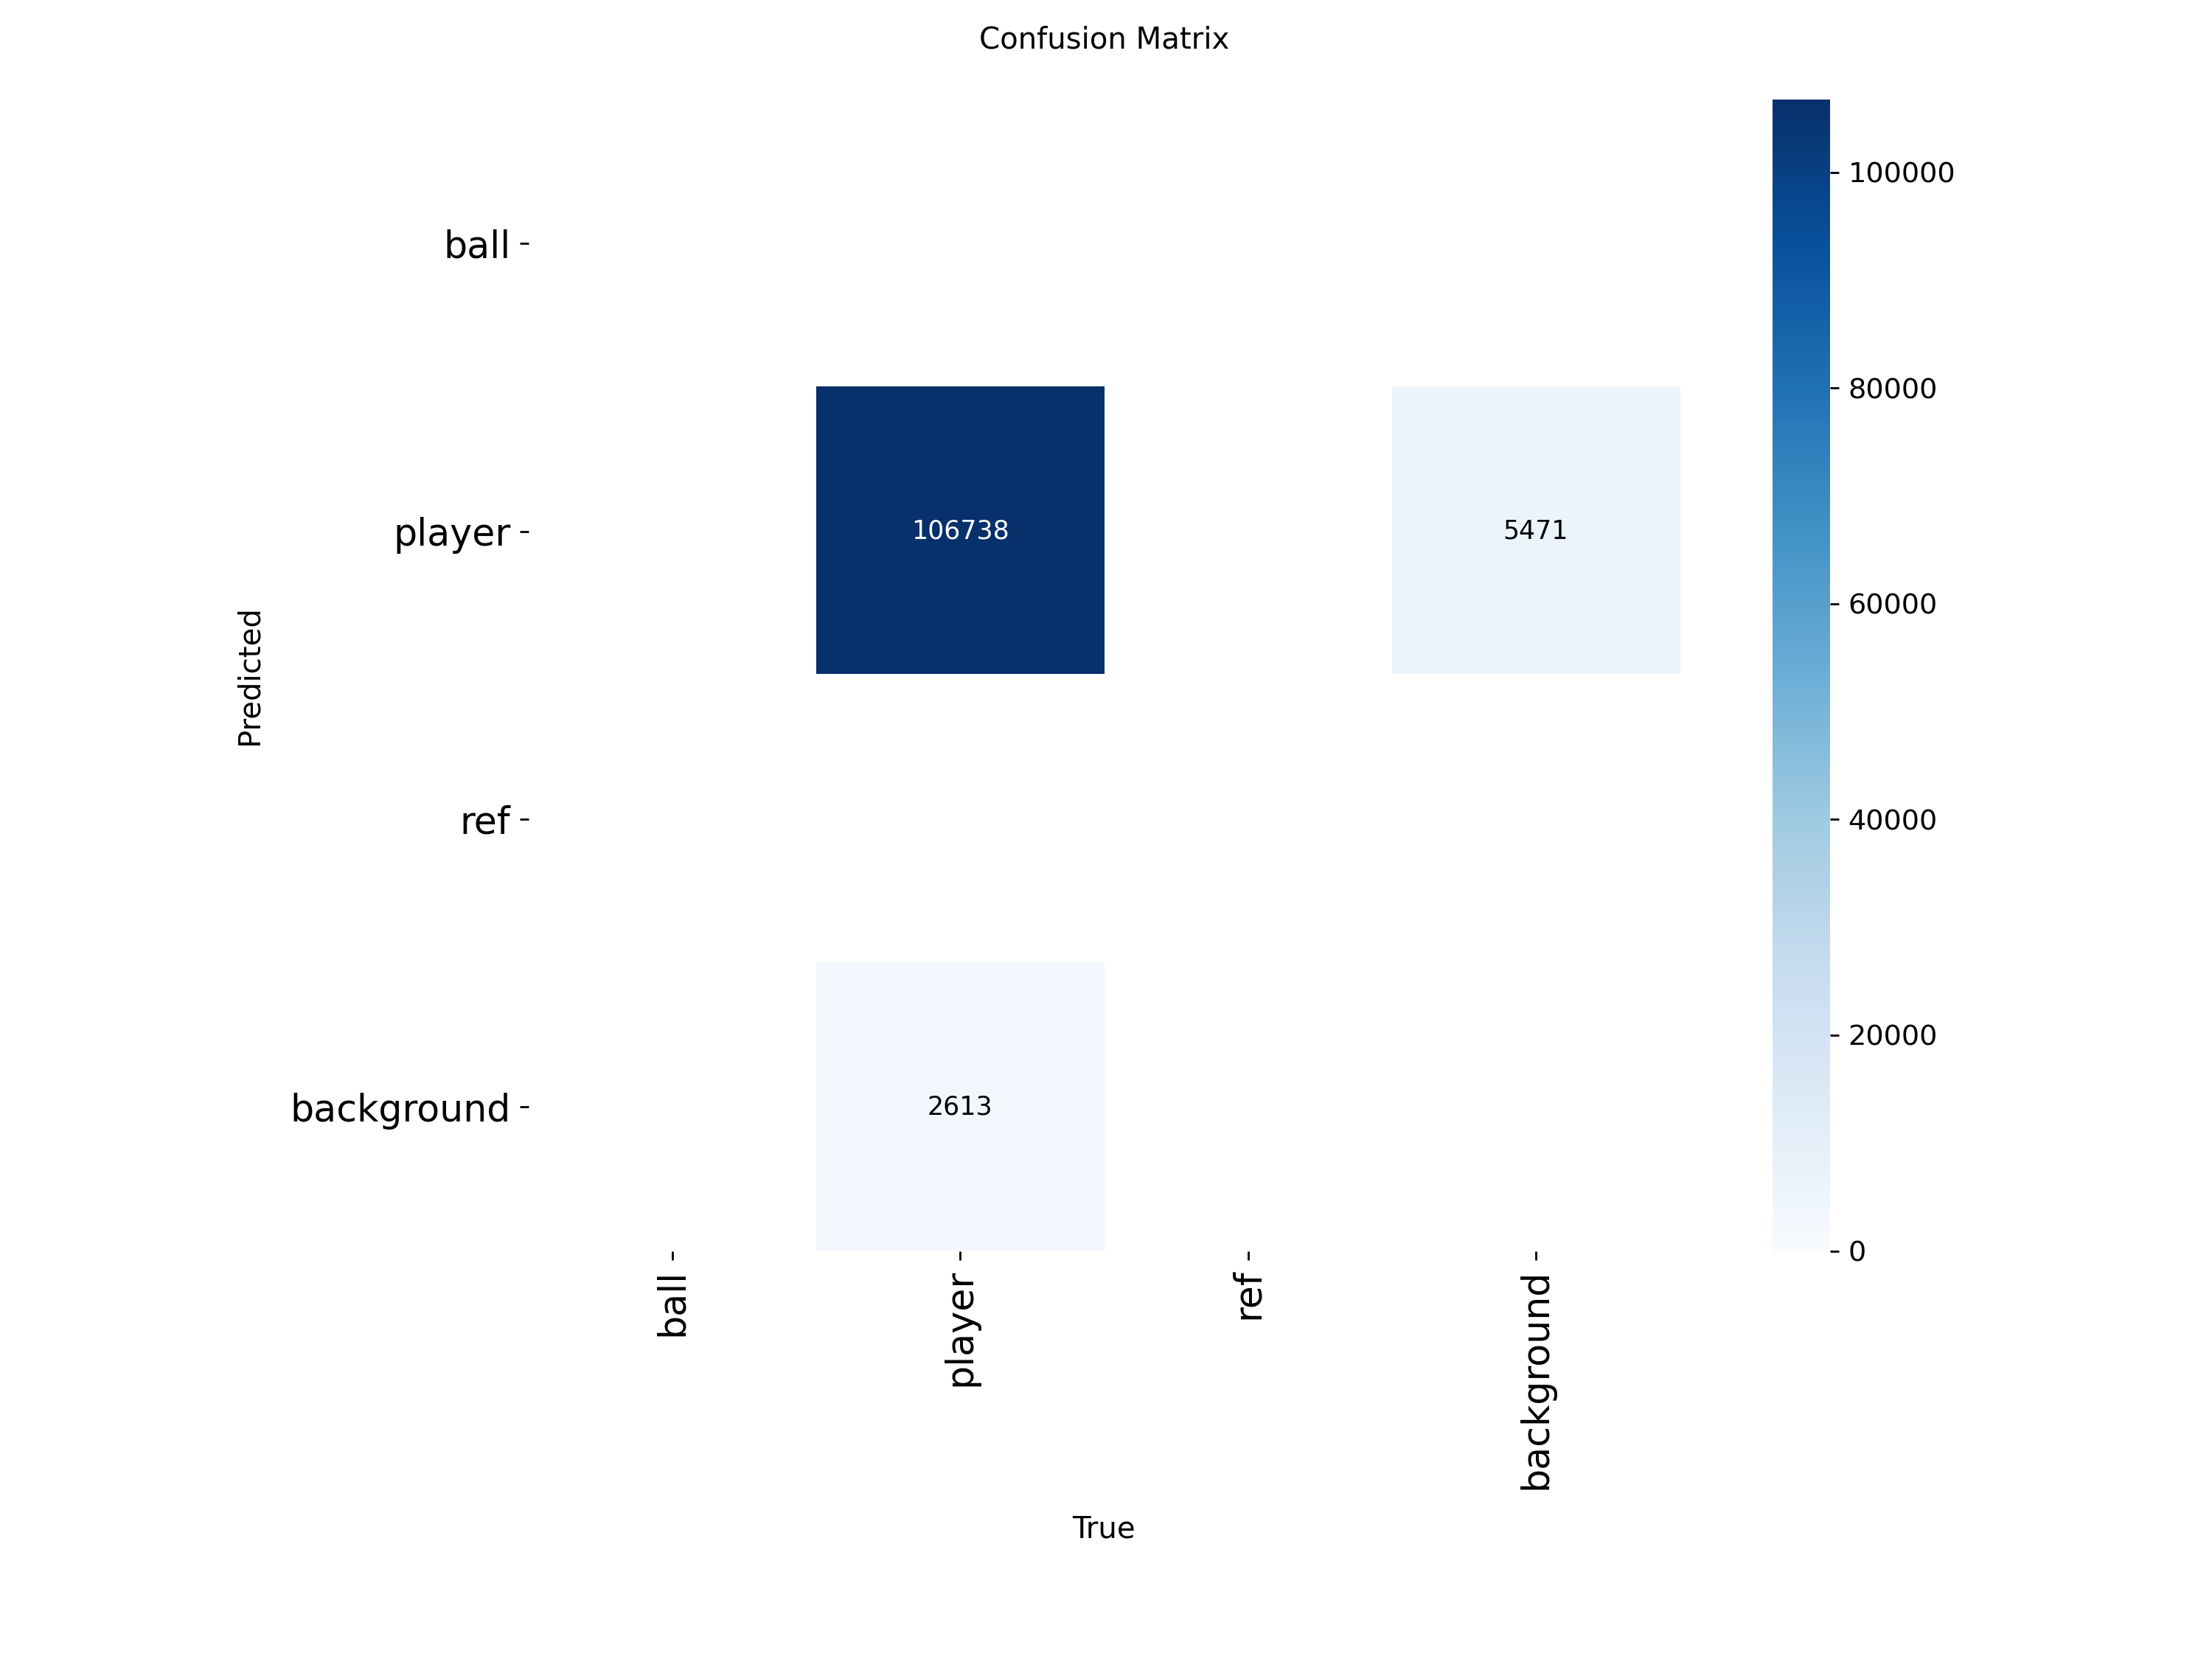
\includegraphics[width=\textwidth]{Imagenes/Propias/confusion_sinteticos.png}
    \small (a) Matriz de confusión en Datos Sintéticos
\end{minipage}

\vspace{0.4cm}

\begin{minipage}{0.55\textwidth}
    \centering
    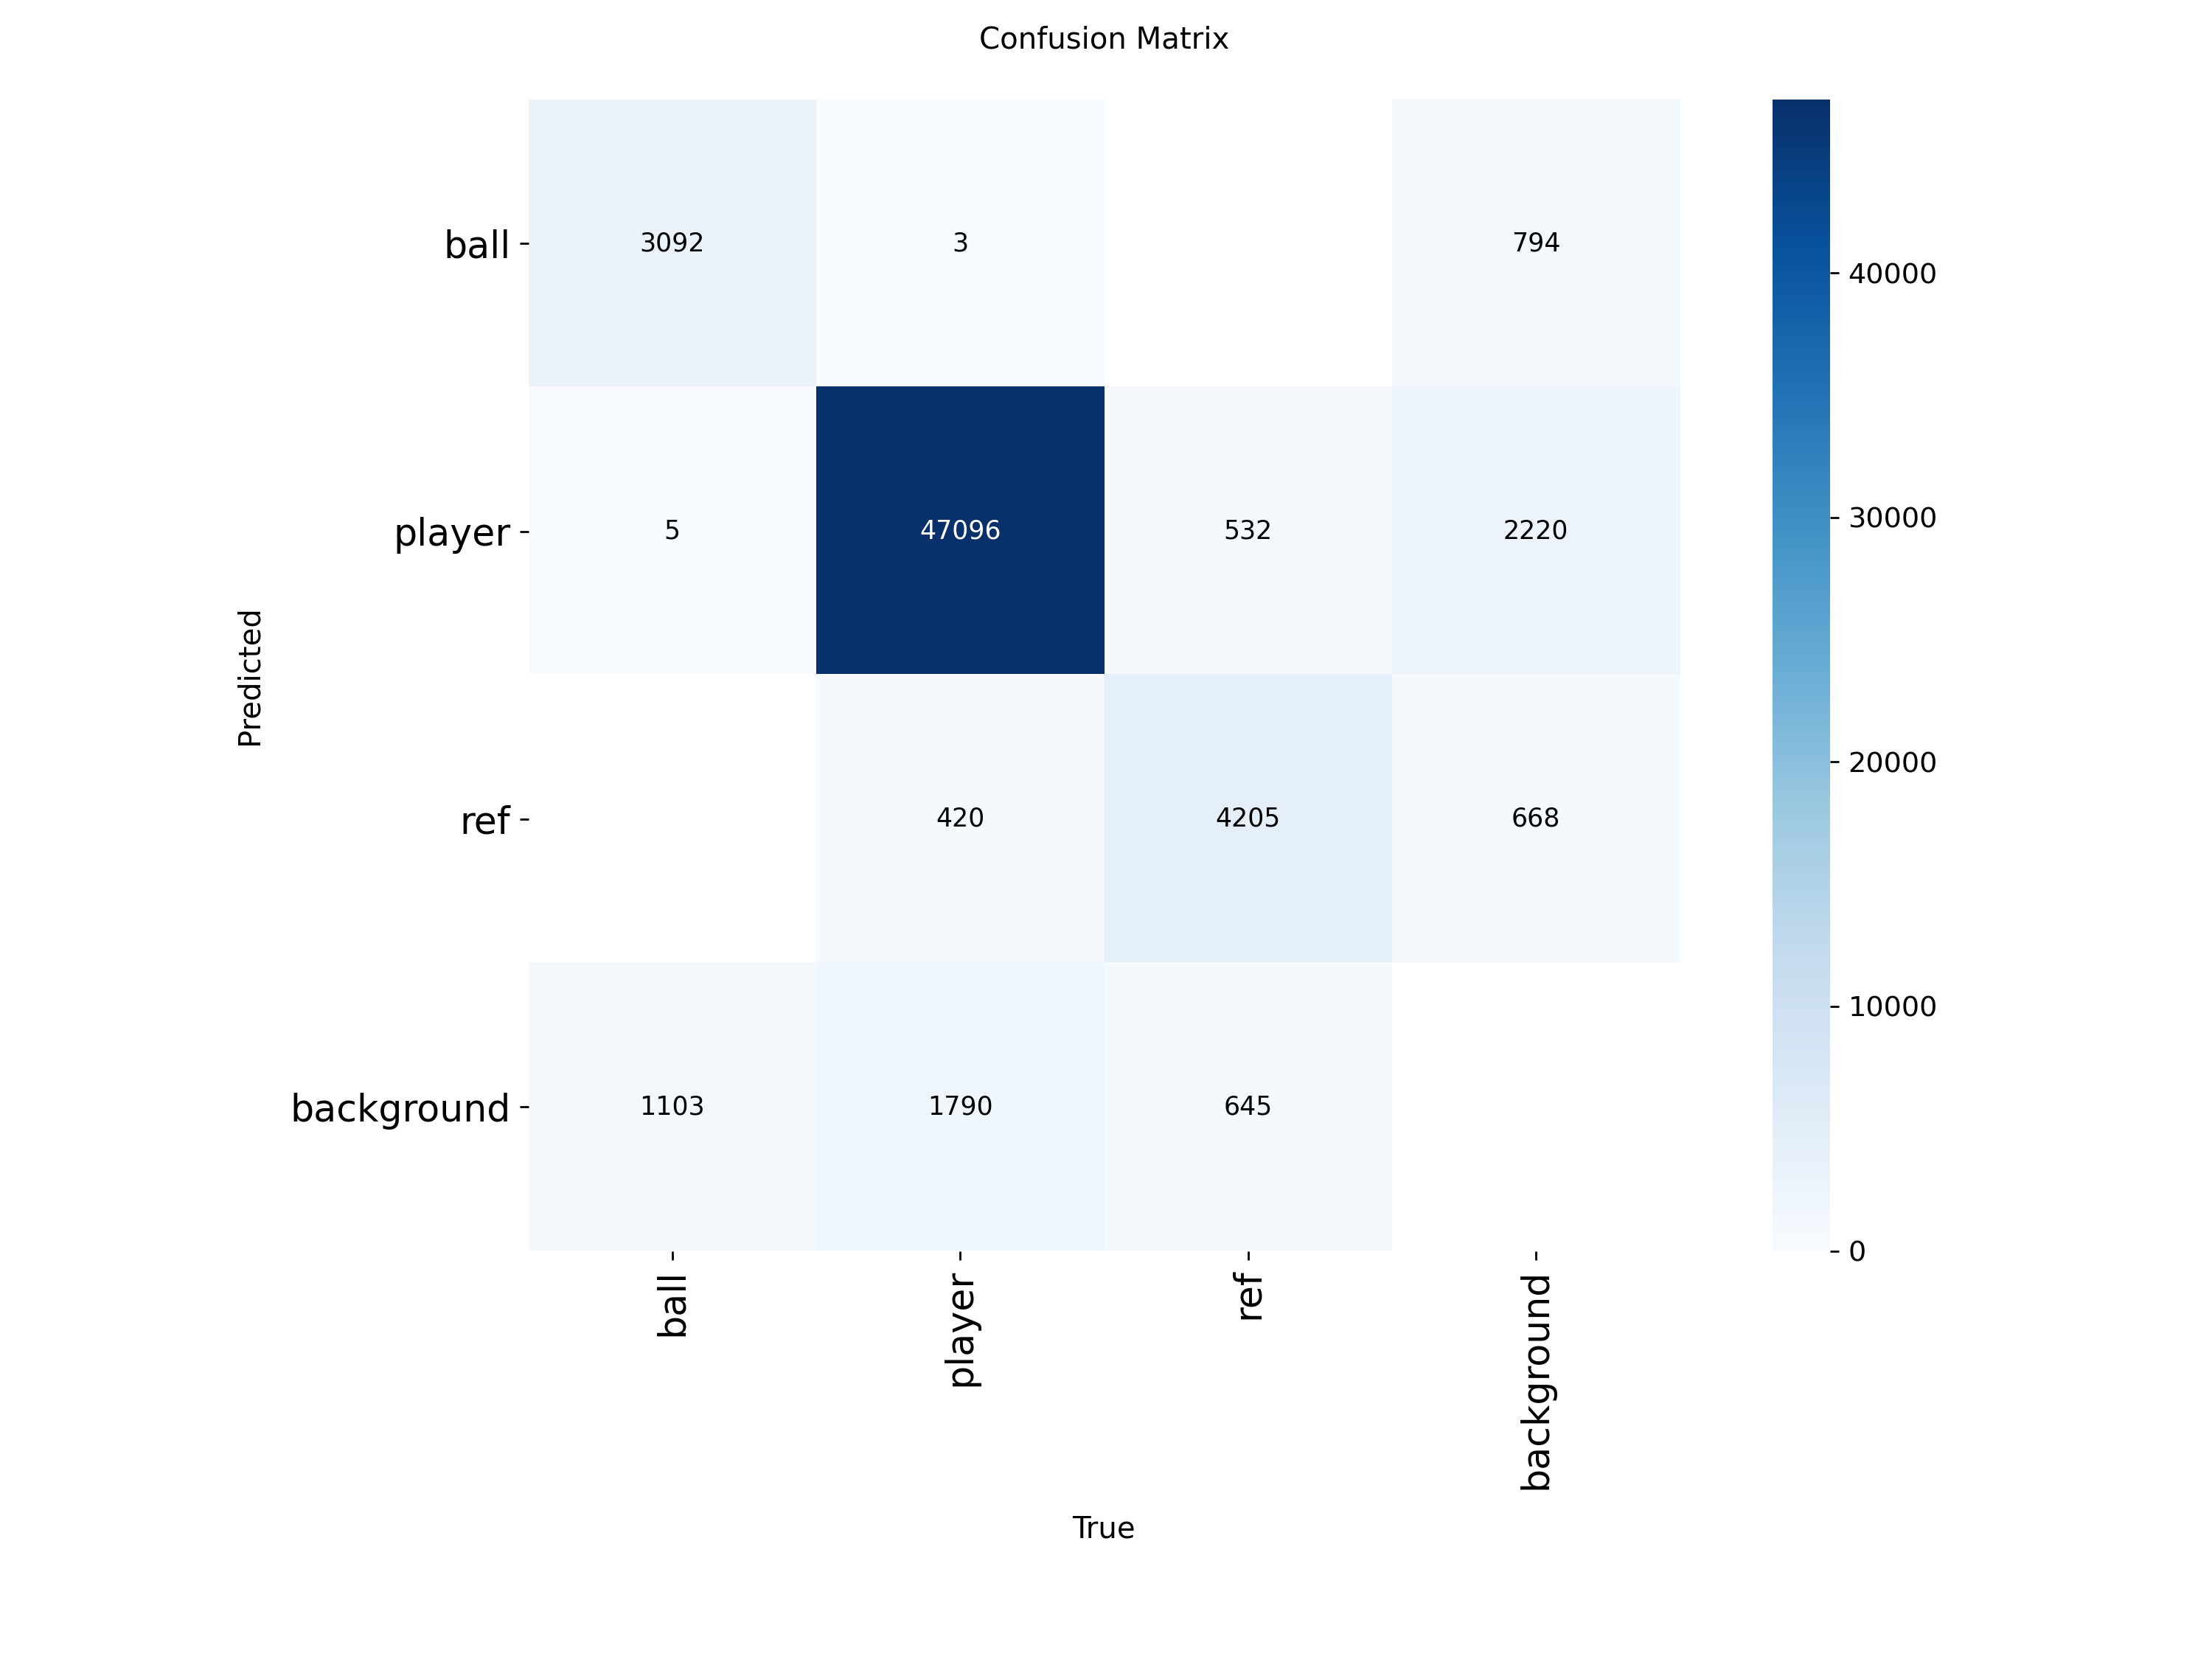
\includegraphics[width=\textwidth]{Imagenes/Propias/confusion_dfl.png}
    \small (b) Matriz de confusión en DFL-Bundesliga.
\end{minipage}

\caption[Matrices de confusión en los datasets de fine-tuning]{
Matrices de confusión en los datasets utilizados durante el \textit{fine-tuning} secuencial. La categoría \texttt{background} no corresponde a una clase entrenada del detector, sino que se incluye en la matriz para representar errores de detección, como objetos reales no detectados o predicciones que no se corresponden con ninguna anotación.
}


\label{fig:confusion_finetuning_compare}
\end{figure}

\subsection{Evaluación sobre la validación de DFL-Bundesliga}

Tras el entrenamiento, se realizó una comparación adicional entre los modelos sobre una misma partición de evaluación: el conjunto de validación de DFL-Bundesliga. El objetivo de esta prueba era comparar ambos detectores bajo un mismo dominio y con las mismas clases de evaluación. Aunque esta partición no se utilizó para actualizar los pesos durante el entrenamiento, no debe interpretarse como un conjunto externo completamente independiente, ya que pertenece al mismo dominio que la segunda fase del \textit{fine-tuning} secuencial.

\subsubsection{Modelos comparados}

En esta evaluación se compararon dos modelos. El primero corresponde al detector afinado directamente sobre el dataset Roboflow fútbol. El segundo corresponde al detector obtenido mediante el proceso secuencial de \textit{fine-tuning}, entrenado primero sobre SoccerSynth-Detection y refinado posteriormente sobre DFL-Bundesliga.

La evaluación se realizó sobre las clases comunes del conjunto de validación: \texttt{ball}, \texttt{player} y \texttt{ref}. La clase \texttt{goalkeeper}, presente en el modelo entrenado con Roboflow fútbol, no se evaluó como categoría independiente, sino que se mapeó a \texttt{player} para mantener una definición de clases común entre ambos modelos.


\subsubsection{Métricas utilizadas}

Las métricas de precisión, recall, F1 e IoU ya se definieron previamente en la \hyperref[subsec:metricas-deteccion-objetos]{Sección~\ref*{subsec:metricas-deteccion-objetos}}. En esta evaluación se utilizan para comparar el comportamiento de los dos detectores sobre la partición de validación de DFL-Bundesliga.

En primer lugar, se analiza el número de instancias reales frente al número de predicciones generadas por cada modelo, como se recoge en la \hyperref[tab:model_comparison_counts]{Tabla~\ref*{tab:model_comparison_counts}}. El número de instancias reales se indica como GT, mientras que el número de predicciones muestra cuántas detecciones produjo cada detector para cada clase. A partir de ambos valores se calcula la tasa de detección, definida como el cociente entre predicciones e instancias reales. Un valor inferior a 1 indica que el modelo tiende a detectar menos objetos de los anotados, mientras que un valor superior a 1 puede indicar mayor cobertura, aunque también riesgo de sobredetección.

La evaluación principal se realiza con un criterio estricto de IoU $\geq 0.50$. Bajo este criterio, una predicción se considera correcta únicamente si la clase coincide con la anotación real y el solape entre ambas cajas supera dicho umbral. A partir de esta correspondencia se calculan precisión, recall y F1 para cada clase, cuyos resultados se muestran en la \hyperref[tab:model_comparison_iou50]{Tabla~\ref*{tab:model_comparison_iou50}}.

Además, se calculan métricas más laxas para analizar la localización aproximada de los objetos, recogidas en la \hyperref[tab:model_comparison_soft]{Tabla~\ref*{tab:model_comparison_soft}}. El recall con IoU $\geq 0.10$ permite comprobar si el modelo detecta el objeto en una zona cercana aunque la caja no encaje con precisión. Esta métrica es útil en fútbol porque algunos objetos, especialmente el balón, pueden detectarse en la zona correcta pero con cajas poco estables. También se incluye un recall basado en centro, que considera correcta una detección si el centro de la caja real cae dentro de alguna caja predicha de la misma clase. Por último, la confianza media resume la seguridad promedio con la que cada modelo emite sus predicciones.


\subsection{Resultados cuantitativos}

La \hyperref[tab:model_comparison_counts]{Tabla~\ref*{tab:model_comparison_counts}} recoge el número de instancias reales y predicciones de cada modelo. La \hyperref[tab:model_comparison_iou50]{Tabla~\ref*{tab:model_comparison_iou50}} muestra la evaluación estricta con IoU $\geq 0.50$, mientras que la \hyperref[tab:model_comparison_soft]{Tabla~\ref*{tab:model_comparison_soft}} incluye métricas más laxas para analizar la localización aproximada de los objetos.

\begin{table}[H]
\centering
\scriptsize
\begin{tabular}{c|c|c|c|c|c}
\textbf{Clase} & \textbf{GT} & \textbf{Pred. Rob.} & \textbf{Pred. Sec.} & \textbf{Tasa Rob.} & \textbf{Tasa Sec.} \\
\hline\hline
\texttt{ball} & 4200 & 1650 & 5111 & 0.3929 & 1.2169 \\
\hline
\texttt{player} & 49570 & 53541 & 51812 & 1.0801 & 1.0452 \\
\hline
\texttt{ref} & 5382 & 5357 & 5503 & 0.9954 & 1.0225 \\
\hline
\end{tabular}
\caption[Instancias y predicciones en la validación de DFL-Bundesliga]{
Número de instancias reales, predicciones y tasa de detección de ambos modelos sobre la partición de validación de DFL-Bundesliga.
}
\label{tab:model_comparison_counts}
\end{table}

\begin{table}[H]
\centering
\scriptsize
\begin{tabular}{c|c|c|c|c|c|c}
\textbf{Clase} & \textbf{Prec. Rob.} & \textbf{Prec. Sec.} & \textbf{Recall Rob.} & \textbf{Recall Sec.} & \textbf{F1 Rob.} & \textbf{F1 Sec.} \\
\hline\hline
\texttt{ball} & 0.6582 & 0.6312 & 0.2586 & 0.7681 & 0.3713 & 0.6929 \\
\hline
\texttt{player} & 0.8642 & 0.9217 & 0.9335 & 0.9633 & 0.8975 & 0.9420 \\
\hline
\texttt{ref} & 0.7000 & 0.8390 & 0.6968 & 0.8579 & 0.6984 & 0.8483 \\
\hline
\end{tabular}
\caption[Comparación estricta con IoU $\geq 0.50$]{
Comparación estricta con IoU $\geq 0.50$ entre el modelo Roboflow y el modelo secuencial SoccerSynth+DFL.
}
\label{tab:model_comparison_iou50}
\end{table}

\begin{table}[H]
\centering
\scriptsize
\renewcommand{\arraystretch}{1.15}
\begin{tabular}{c|c|c|c|c|c|c}
\textbf{Clase} & \textbf{R@0.10 Rob.} & \textbf{R@0.10 Sec.} & \textbf{Centro Rob.} & \textbf{Centro Sec.} & \textbf{Conf. Rob.} & \textbf{Conf. Sec.} \\
\hline\hline
\texttt{ball} & 0.3114 & 0.8340 & 0.3129 & 0.8357 & 0.3522 & 0.5078 \\
\hline
\texttt{player} & 0.9427 & 0.9664 & 0.9743 & 0.9871 & 0.7394 & 0.7942 \\
\hline
\texttt{ref} & 0.7150 & 0.8610 & 0.7179 & 0.8634 & 0.6122 & 0.6951 \\
\hline
\end{tabular}
\caption[Métricas laxas en la validación de DFL-Bundesliga]{
Métricas laxas y confianza media de ambos modelos sobre la partición de validación de DFL-Bundesliga. R@0.10 indica recall con IoU $\geq 0.10$, Centro indica recall basado en centro, Rob. corresponde al modelo entrenado sobre Roboflow fútbol y Sec. al modelo secuencial SoccerSynth+DFL.
}
\label{tab:model_comparison_soft}
\end{table}

\subsection{Interpretación de los Resultados}
Los resultados muestran una mejora clara del modelo secuencial SoccerSynth+DFL sobre la partición de validación de DFL-Bundesliga. La diferencia es especialmente notable en la clase \texttt{ball}: el modelo Roboflow detecta 1650 balones frente a 4200 instancias reales, con un recall estricto de 0.2586, mientras que el modelo secuencial produce 5111 predicciones y alcanza un recall estricto de 0.7681. Aunque su precisión en balón es ligeramente menor, el aumento de cobertura resulta muy relevante para el sistema, ya que el balón es uno de los objetos más pequeños y difíciles de detectar.

En la clase \texttt{player}, el modelo secuencial también mejora las métricas principales, pasando de un F1 de 0.8975 a 0.9420. En la clase \texttt{ref}, la mejora es igualmente consistente, con un aumento del F1 de 0.6984 a 0.8483. Además, las métricas laxas muestran que el modelo secuencial localiza mejor los objetos incluso cuando se relaja el criterio de solape, lo que sugiere una mayor robustez espacial en este dominio.

Estos resultados indican que la estrategia de adaptación con datos sintéticos seguida de refinamiento sobre DFL-Bundesliga es más adecuada para este escenario que el entrenamiento directo sobre el dataset pequeño de Roboflow. No obstante, esta comparación debe interpretarse teniendo en cuenta que se realiza sobre la partición de validación de DFL-Bundesliga, por lo que no constituye una evaluación externa completamente independiente.

La decisión final del detector no debe basarse únicamente en estas métricas de detección aislada. El sistema completo depende también del comportamiento del tracking, de la estabilidad temporal de las identidades y de cómo se comporta el modelo sobre vídeos reales, donde aparecen compresión, movimiento de cámara, cambios de plano y oclusiones. Por este motivo, aunque esta comparación favorece al modelo sintético+DFL, la decisión final se deja abierta hasta completar las pruebas de tracking sobre vídeo real.
\section{Calibración del campo y proyección a coordenadas métricas}
\label{sec:calibracion-campo-proyeccion-metricas}

En la \hyperref[sec:homografia-tecnologias]{Sección~\ref*{sec:homografia-tecnologias}} se introdujo el concepto de homografía y se describió PnLCalib como método para estimar la calibración geométrica del campo en vídeo broadcast. En esta sección se resume cómo se ha integrado dicha calibración dentro del sistema y, especialmente, qué estrategias de robustez han sido necesarias para poder usar la homografía como una señal fiable dentro del pipeline.

\subsection{Modelo utilizado y salida geométrica}

En este proyecto se utiliza PnLCalib en modo inferencia, con sus pesos pre-entrenados publicados por los autores en el repositorio oficial del proyecto \citep{PnLCalibRepo2024}, para estimar en cada frame la geometría del campo visible. A partir de las predicciones de puntos y líneas del terreno se obtiene una homografía $H_t$ que permite proyectar coordenadas en píxeles $(u,v)$ a coordenadas 2D sobre el plano del campo $(x,y)$, expresadas en unidades métricas.

La \hyperref[fig:calibracion-proyeccion-campo]{Figura~\ref*{fig:calibracion-proyeccion-campo}} ilustra este proceso. En la imagen original se muestran los puntos de referencia detectados sobre el terreno de juego, mientras que la vista cenital resultante permite visualizar la proyección de la escena sobre el plano del campo.

\begin{figure}[H]
\centering

\begin{minipage}{0.9\textwidth}
    \centering
    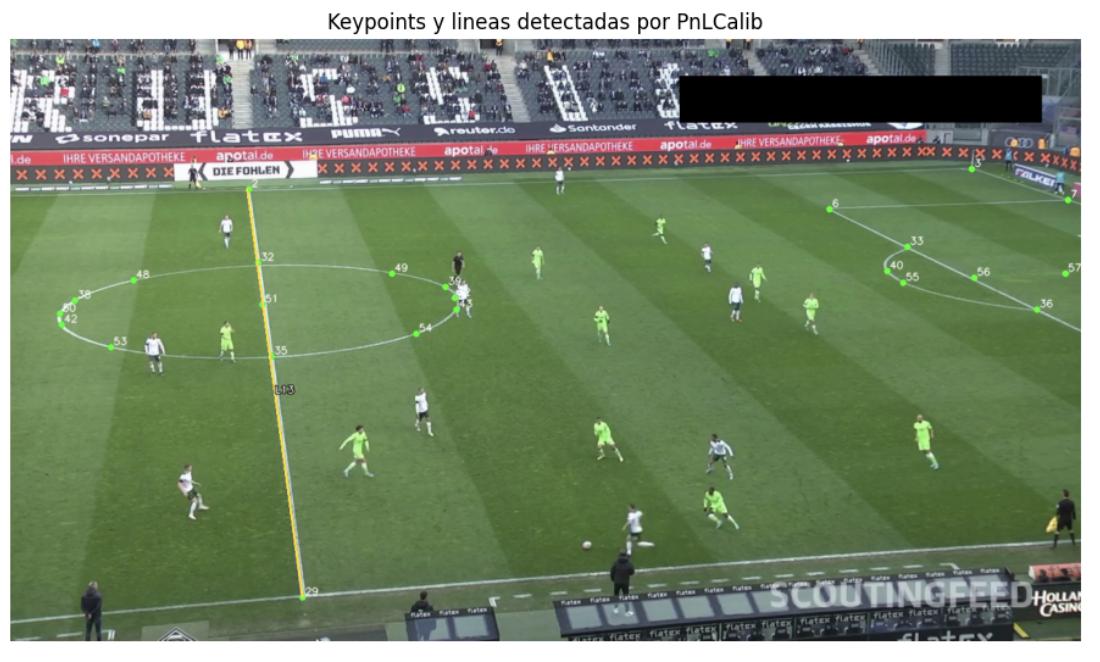
\includegraphics[width=\textwidth]{Imagenes/Propias/Puntos_referencia.png}
    \small \textbf{(a)} Puntos de referencia detectados sobre la imagen broadcast.
\end{minipage}

\vspace{0.4cm}

\begin{minipage}{0.9\textwidth}
    \centering
    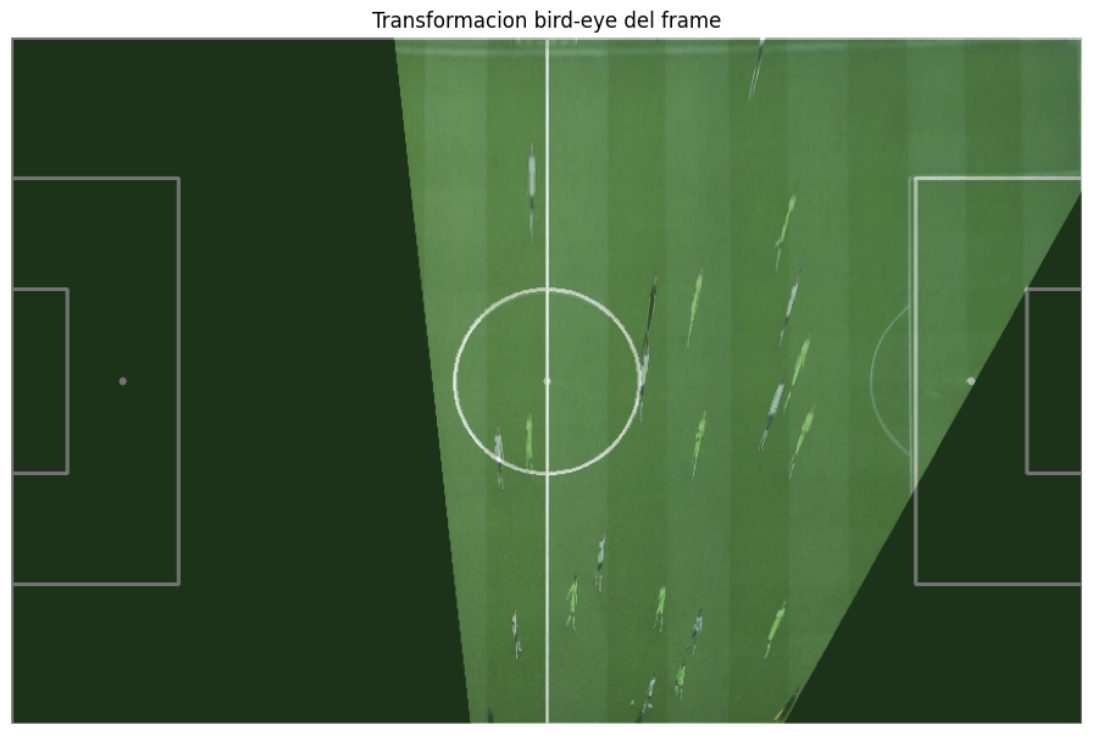
\includegraphics[width=\textwidth]{Imagenes/Propias/Bird_eye.png}
    \small \textbf{(b)} Proyección resultante en vista cenital del terreno de juego.
\end{minipage}

\caption[Calibración geométrica y proyección al plano del campo]{
Ejemplo de calibración geométrica del campo mediante PnLCalib. En (a) se muestran las referencias detectadas sobre la imagen broadcast y, en (b), la proyección de la escena sobre una representación 2D del terreno de juego.
}
\label{fig:calibracion-proyeccion-campo}
\end{figure}

Para proyectar la posición de un jugador no se utiliza el centro de su \textit{bounding box}, sino un punto que aproxima el contacto con el césped. En concreto, se emplea el punto central inferior de la caja, ligeramente desplazado hacia arriba:
\[
x = \frac{x_1 + x_2}{2}
\qquad
y = y_2 - 0.04 \cdot (y_2 - y_1)
\]
donde $(x_1,y_1,x_2,y_2)$ son las coordenadas de la \textit{bounding box}. Este punto se transforma mediante la homografía para obtener una posición $(x,y)$ en el campo.

La configuración de esta fase se resume en la \hyperref[tab:hiperparametros-referencia]{Tabla~\ref*{tab:hiperparametros-referencia}}, donde se recogen los parámetros utilizados por el módulo de proyección y sobre los que se irá hablando a lo largo de la sección.

\begin{table}[htbp]
\centering
\scriptsize
\setlength{\tabcolsep}{3pt}
\renewcommand{\arraystretch}{1.10}
\begin{tabularx}{\textwidth}{
>{\raggedright\arraybackslash}p{2.5cm}
>{\raggedright\arraybackslash}p{3.3cm}
>{\raggedright\arraybackslash}p{1.4cm}
>{\raggedright\arraybackslash}X
}
\toprule
\textbf{Bloque} & \textbf{Parámetro} & \textbf{Valor} & \textbf{Uso en pipeline} \\
\midrule

Redimensionado y punto de apoyo &
\texttt{bottom\_offset\_ratio} &
\texttt{0.04} &
Fija el desplazamiento vertical del punto proyectado sobre el césped. \\

\midrule

Umbrales base de inferencia &
\texttt{kp\_threshold} &
\texttt{0.30} &
Controla qué puntos de referencia se aceptan inicialmente. \\

&
\texttt{line\_threshold} &
\texttt{0.60} &
Controla qué líneas del campo se aceptan inicialmente. \\

&
\texttt{pnl\_refine} &
\texttt{false} &
Desactiva el refinamiento PnL adicional en esta configuración. \\

\midrule

Suavizado temporal &
\texttt{temporal\_blend} &
\texttt{0.20} &
Mezcla la homografía del frame actual con la anterior si la solución suavizada mantiene la calidad requerida. \\

\midrule

Búsqueda adaptativa &
\texttt{adaptive\_thresholds} &
\texttt{true} &
Activa varios intentos de calibración relajando umbrales. \\

&
\texttt{adaptive\_max\_attempts} &
\texttt{4} &
Número máximo de intentos por frame. \\

&
\texttt{adaptive\_kp\_step} &
\texttt{0.02} &
Reducción progresiva del umbral de puntos. \\

&
\texttt{adaptive\_line\_step} &
\texttt{0.05} &
Reducción progresiva del umbral de líneas. \\

&
\texttt{min. kp/line thresholds} &
\texttt{0.28/0.55} &
Límites inferiores hasta los que se relajan los umbrales. \\

\midrule

Soporte mínimo &
\texttt{min\_visible\_kp} &
\texttt{7} &
Número mínimo de puntos visibles requerido para aceptar una calibración. \\

&
\texttt{min\_visible\_lines} &
\texttt{1} &
Número mínimo de líneas visibles requerido para aceptar una calibración. \\

\midrule

Validación global &
\texttt{val\_score\_th} &
\texttt{0.56} &
Umbral mínimo del score compuesto de validación. \\

&
\texttt{val\_geometry\_fit\_min} &
\texttt{0.38} &
Mínimo requerido para la calidad del ajuste geométrico. \\

&
\texttt{val\_support\_quality\_min} &
\texttt{0.31} &
Mínimo requerido para la calidad del soporte geométrico. \\

&
\texttt{val\_coverage\_quality\_min} &
\texttt{0.18} &
Mínimo requerido para la cobertura de referencias. \\

\midrule

Validación geométrica &
\texttt{val\_reproj\_err\_px} &
\texttt{8.0} &
Rechaza soluciones con error de reproyección elevado. \\

&
\texttt{val\_H\_cond\_th} &
\texttt{1e8} &
Descarta homografías mal condicionadas. \\

&
\texttt{val\_kp\_world\_err\_m} &
\texttt{3.0} &
Limita el error métrico permitido en puntos. \\

&
\texttt{val\_line\_world\_err\_m} &
\texttt{4.0} &
Limita el error métrico permitido en líneas. \\

\midrule

Objetivos de cobertura &
\texttt{val\_target\_visible\_kp} &
\texttt{9} &
Objetivo de puntos visibles para considerar una calibración estable. \\

&
\texttt{val\_target\_visible\_lines} &
\texttt{4} &
Objetivo de líneas visibles. \\

&
\texttt{val\_target\_hull\_area} &
\texttt{0.18} &
Mide la cobertura espacial de los puntos en la imagen. \\

&
\texttt{val\_target\_x\_span} &
\texttt{0.55} &
Mide la extensión horizontal de las referencias. \\

&
\texttt{val\_target\_y\_span} &
\texttt{0.40} &
Mide la extensión vertical de las referencias. \\

&
\texttt{val\_target\_field\_cov} &
\texttt{0.20} &
Mide si las referencias cubren suficiente campo para estimar una homografía estable. \\

\bottomrule
\end{tabularx}

\caption[Hiperparámetros de calibración y proyección métrica]{
Hiperparámetros principales de la fase de calibración geométrica y proyección a coordenadas métricas.}
\label{tab:hiperparametros-referencia}
\end{table}

El valor final de estos hiperparámetros recogidos en la tabla se decidió mediante depuración iterativa y pruebas visuales sobre el vídeo de referencia. Este proceso de depuración se describe en la \hyperref[sec:evaluacion-heuristica-depuracion]{Sección~\ref*{sec:evaluacion-heuristica-depuracion}}.

\subsection{Problema de estabilidad: \textit{jitter} y sensibilidad a umbrales}

Durante las primeras pruebas se observó que la homografía estimada frame a frame era una señal poco estable: pequeñas variaciones en los puntos/líneas detectados producían cambios apreciables en la proyección, generando \textit{jitter} (vibración) tanto en la reconstrucción del campo como en las trayectorias proyectadas de los jugadores.

Este comportamiento ocurría principalmente con planos cerrados (esquinas o área), cuando la cámara realiza paneos o zooms rápidos, etc. 

Además, el método depende de umbrales de confianza para decidir qué puntos y líneas se consideran observados. En la práctica, fijar estos umbrales de forma única para todos los vídeos resulta difícil: con umbrales altos se obtienen menos referencias y muchos frames quedan sin homografía, mientras que con umbrales bajos se aceptan referencias ruidosas que degradan la calibración. Por tanto, la elección de umbrales tiene un componente arbitrario y el ``mejor'' valor depende del vídeo (calidad, resolución, iluminación y tipo de plano).

\subsection{Selección robusta de homografía: umbrales adaptativos y validación}

Para mejorar la robustez, se implementó una búsqueda por intentos con umbrales adaptativos sobre puntos clave y líneas. En cada frame se parte de una configuración base y se generan varios intentos relajando progresivamente los umbrales (hasta mínimos definidos), con el objetivo de aumentar el soporte geométrico en escenas difíciles.

El sistema evalúa todos los intentos y selecciona el mejor según un criterio lexicográfico: (i) aceptación de calidad, (ii) \textit{quality score} global y, en caso de empate, (iii) submétricas de ajuste geométrico, soporte y cobertura. Si ningún intento resulta aceptable, el frame se marca como no proyectable.

Esta estrategia permite adaptarse a distintos tipos de plano dentro del mismo partido (por ejemplo, plano general frente a plano cercano), y reduce la necesidad de calibrar manualmente umbrales por vídeo.

\subsubsection{Métricas de calidad y criterio de aceptación}

La homografía estimada no se utiliza de forma incondicional: se valida su calidad antes de habilitar su uso en tracking. El criterio que define la calidad de una homografía viene dado por la combinación de tres señales en un \textit{score} compuesto:
\begin{itemize}
    \item \textbf{Ajuste geométrico (\textit{geometry fit}):} incluye error de reproyección y chequeos de consistencia geométrica.
    \item \textbf{Soporte de referencias (\textit{support quality}):} cantidad y fiabilidad de puntos/líneas detectados.
    \item \textbf{Cobertura (\textit{coverage quality}):} distribución espacial/semántica de referencias para evitar soluciones concentradas o débiles.
\end{itemize}

Además del \textit{score} global, se aplican umbrales mínimos por submétrica y checks numéricos. Solo si el intento supera estos criterios se marca como aceptable para uso en tracking.

\subsubsection{Definición matemática de las métricas de calidad}

Sea un intento de calibración en un frame dado. Definimos funciones de normalización:
\[
clip(x)=\min(1,\max(0,x)),
\qquad
s_{\text{inv}}(e;\tau)=\frac{\tau}{\tau+e}
\]
\[
s_{\text{range}}(v;v_{\min},v_{\text{obj}})=
\mathrm{clip}\!\left(\frac{v-v_{\min}}{v_{\text{obj}}-v_{\min}}\right)
\]

Aquí, \({clip}\) acota cualquier valor al intervalo \([0,1]\), 
\(s_{\text{inv}}\) transforma un error \(e\) en una puntuación donde un valor mayor indica mejor calidad, y \(\tau\) controla la sensibilidad de esa transformación (en particular, \(s_{\text{inv}}=0.5\) cuando \(e=\tau\)), y \(s_{\text{range}}\) normaliza una magnitud \(v\) entre un mínimo y un objetivo, saturando el resultado en \([0,1]\).


Todas las submétricas se llevan a \([0,1]\), donde \(1\) es mejor.

\paragraph{1) Ajuste geométrico}
\[
G = 0.35\,s_{\text{rep}} + 0.15\,s_{\text{cond}} + 0.30\,s_{\text{kp-align}} + 0.20\,s_{\text{line-align}}
\]
con:
\[
s_{\text{rep}} = s_{\text{inv}}(e_{\text{rep}};\tau_{\text{rep}}),
\qquad
s_{\text{cond}}=
\mathrm{clip}\!\left(
1-\frac{\log_{10}(\kappa(H))}{\log_{10}(\kappa_{\max})}
\right),
\]
\[
s_{\text{kp-align}} = s_{\text{inv}}(e_{\text{kp-world}};\tau_{\text{kp-world}}),
\qquad
s_{\text{line-align}} = s_{\text{inv}}(e_{\text{line-world}};\tau_{\text{line-world}}).
\]

Donde \(e_{\text{rep}}\) es el error de reproyección devuelto por PnLCalib, \(\kappa(H)\) es el número de condición de la homografía \(H\), y \(e_{\text{kp-world}}\), \(e_{\text{line-world}}\) son errores medianos en metros tras proyectar puntos y líneas al campo. Los umbrales \(\tau_{\text{rep}}\), \(\kappa_{\max}\), \(\tau_{\text{kp-world}}\) y \(\tau_{\text{line-world}}\) corresponden a los valores de la Tabla~\ref{tab:hiperparametros-referencia} (respectivamente: \textit{val\_reproj\_err\_px}, \textit{val\_H\_cond\_th}, \textit{val\_kp\_world\_err\_m}, \textit{val\_line\_world\_err\_m}).

\(s_{\text{rep}}\) mide la consistencia global de la proyección en imagen (qué bien se reinyectan las referencias detectadas), \(s_{\text{cond}}\) mide la estabilidad numérica de la homografía estimada penalizando matrices mal condicionadas, \(s_{\text{kp-align}}\) mide la coherencia métrica de los puntos clave proyectados sobre el campo, y \(s_{\text{line-align}}\) mide la coherencia métrica de las líneas proyectadas en el plano del campo. En conjunto, estas submétricas capturan tanto el ajuste visual en imagen como la validez geométrica y la estabilidad numérica de la solución en coordenadas de juego.


\paragraph{2) Calidad del soporte de las referencias}
\[
S =
0.25\,s_{\text{kp-count}}
+ 0.20\,s_{\text{line-count}}
+ 0.15\,s_{\text{kp-conf}}
+ 0.10\,s_{\text{line-conf}}
+ 0.15\,s_{\text{kp-family}}
+ 0.15\,s_{\text{line-family}}.
\]

con:
\[
s_{\text{kp-count}}=
s_{\text{range}}(N_{kp};N_{kp}^{\min},N_{kp}^{obj}),\qquad
s_{\text{line-count}}=
s_{\text{range}}(N_{line};N_{line}^{\min},N_{line}^{obj}),
\]
\[
s_{\text{kp-conf}}=\frac{1}{N_{kp}}\sum_{i=1}^{N_{kp}} c^{kp}_i,\qquad
s_{\text{line-conf}}=\frac{1}{N_{line}}\sum_{j=1}^{N_{line}} c^{line}_j,
\]
\[
s_{\text{kp-family}}
=
\frac{1}{2}\left(\frac{B_x}{3}+\frac{B_y}{3}\right),
\]
\[
s_{\text{line-family}}
=
\mathrm{clip}\!\left(\frac{F_{\text{line}}}{3}\right).
\]

Donde \(N_{kp}\) y \(N_{line}\) son el número de \textit{keypoints} y líneas visibles; \(c^{kp}_i\) y \(c^{line}_j\) son sus confianzas individuales (devueltas por PnLCalib); \(B_x\) y \(B_y\) son el número de bandas ocupadas por los \textit{keypoints} en los ejes longitudinal y transversal del campo, tras dividir cada eje en tres intervalos; y \(F_{\text{line}}\) es el número de familias geométricas de líneas observadas, distinguiendo entre horizontales, verticales y estructura de portería.

Los umbrales y objetivos \(N_{kp}^{\min}\), \(N_{line}^{\min}\), \(N_{kp}^{obj}\) y \(N_{line}^{obj}\) corresponden a los valores de la Tabla~\ref{tab:hiperparametros-referencia} (respectivamente: \textit{min\_visible\_kp}, \textit{min\_visible\_lines}, \textit{val\_target\_visible\_kp}, \textit{val\_target\_visible\_lines}).

En esta puntuación, \(s_{\text{kp-count}}\) y \(s_{\text{line-count}}\) miden suficiencia de evidencia, \(s_{\text{kp-conf}}\) y \(s_{\text{line-conf}}\) miden fiabilidad media de las detecciones, \(s_{\text{kp-family}}\) mide si los \textit{keypoints} cubren zonas distintas del campo, y \(s_{\text{line-family}}\) mide si las líneas observadas pertenecen a familias geométricas variadas. En conjunto, estas submétricas intentan captar si la calibración se apoya en referencias no solo numerosas y fiables, sino también diversas.

\paragraph{3) Calidad de la cobertura del campo}
\[
C = 0.40\,s_{\text{img-hull}} + 0.20\,s_{\text{field-hull}} + 0.20\,s_{x\text{-span}} + 0.20\,s_{y\text{-span}}
\]
con:
\[
s_{\text{img-hull}}=\mathrm{clip}\!\left(\frac{A_{\text{img-hull}}}{A_{\text{img-hull}}^{\text{obj}}}\right),\qquad
s_{\text{field-hull}}=\mathrm{clip}\!\left(\frac{A_{\text{field-hull}}}{A_{\text{field-hull}}^{\text{obj}}}\right),
\]
\[
s_{x\text{-span}}=\mathrm{clip}\!\left(\frac{p_{x\text{-span}}}{p_{x\text{-span}}^{\text{obj}}}\right),\qquad
s_{y\text{-span}}=\mathrm{clip}\!\left(\frac{p_{y\text{-span}}}{p_{y\text{-span}}^{\text{obj}}}\right).
\]

Donde \(A_{\text{img-hull}}\) es la fracción de área del casco convexo de las referencias en imagen respecto al área total del frame; \(A_{\text{field-hull}}\) es la fracción de área del casco convexo de las referencias proyectadas en el campo respecto al área total del terreno de juego; y \(p_{x\text{-span}}\), \(p_{y\text{-span}}\) son las fracciones del ancho y del alto de la imagen cubiertas por la separación entre la referencia más extrema a izquierda/derecha y la más extrema arriba/abajo, respectivamente.

Los objetivos \(A_{\text{img-hull}}^{\text{obj}}\), \(A_{\text{field-hull}}^{\text{obj}}\), \(p_{x\text{-span}}^{\text{obj}}\) y \(p_{y\text{-span}}^{\text{obj}}\) corresponden a los valores de la Tabla~\ref{tab:hiperparametros-referencia} (respectivamente: \textit{val\_target\_hull\_area}, \textit{val\_target\_field\_cov}, \textit{val\_target\_} \textit{x\_span}, \textit{val\_target\_y\_span}).

En esta puntuación, \(s_{\text{img-hull}}\) mide cuánta superficie útil del frame queda anclada por referencias, \(s_{\text{field-hull}}\) mide su cobertura geométrica tras proyectarlas al plano del campo, y \(s_{x\text{-span}}\), \(s_{y\text{-span}}\) miden cuánto se extienden dichas referencias a lo ancho y a lo alto de la imagen. En conjunto, estas submétricas evalúan si la calibración está soportada por una cobertura amplia y bien distribuida.

\paragraph{Score final y criterio de aceptación:}

Si existe una homografía candidata válida, se calcula una puntuación global como combinación ponderada de las tres métricas anteriores:
\[
Q = 0.45\,G + 0.30\,S + 0.25\,C.
\]

Los umbrales de aceptación sobre estas métricas vienen dados por:
\[
G \ge G_{\min},\quad S \ge S_{\min},\quad C \ge C_{\min},\quad Q \ge Q_{\min},
\]
donde \(G_{\min}\), \(S_{\min}\), \(C_{\min}\) y \(Q_{\min}\) corresponden a los valores de la Tabla~\ref{tab:hiperparametros-referencia} (respectivamente: \textit{val\_geometry\_fit\_min}, \textit{val\_support\_quality\_min}, \textit{val\_coverage\_quality\_min}, \textit{val\_score\_th}).

Sin embargo, la aceptación final no depende solo de estas puntuaciones agregadas. Además, se aplican comprobaciones duras de validez: debe existir una homografía estimada, esta debe ser numéricamente válida y estar suficientemente bien condicionada, y el frame debe alcanzar al menos los mínimos de referencias visibles \(N_{kp}^{\min}\) y \(N_{line}^{\min}\). Por tanto, una solución puede obtener valores altos de \(G\), \(S\), \(C\) y \(Q\), pero aun así ser rechazada si falla alguna de estas condiciones duras.

\subsection{Suavizado temporal}

Incluso con homografías aceptables, puede existir variación frame a frame. Para reducir vibraciones se aplica un suavizado temporal opcional:
\[
H_t^{blend}=\alpha H_{t-1} + (1-\alpha)H_t^{raw}, \quad \alpha=0.20
\]

En la implementación, el resultado suavizado se conserva únicamente si también supera la validación de calidad y no reduce el \textit{quality score} frente a la solución no suavizada.

\subsection{Fallo controlado: \textit{fallback} cuando no hay homografía}

Por último, cuando no se consigue una homografía fiable, el pipeline no se detiene: se descarta la proyección métrica en ese frame y las fases posteriores continúan trabajando en coordenadas de imagen. Esta decisión evita que una calibración errónea contamine el resto del sistema.

En la \hyperref[fig:homography_frame]{Figura~\ref*{fig:homography_frame}} se muestra un ejemplo visual de la salida de esta fase para un frame del vídeo de prueba. En el panel de la izquierda aparecen las detecciones, los puntos y las líneas de referencia encontrados. En el de la derecha se muestra cómo quedan ubicadas las detecciones sobre el campo tras aplicar la homografía. El vídeo del resultado completo puede consultarse en \url{https://github.com/hectorgarciaa/narrador-futbol/output/homography/best/20260516_180637/homography.mp4}.
\begin{figure}[h]
    \centering
    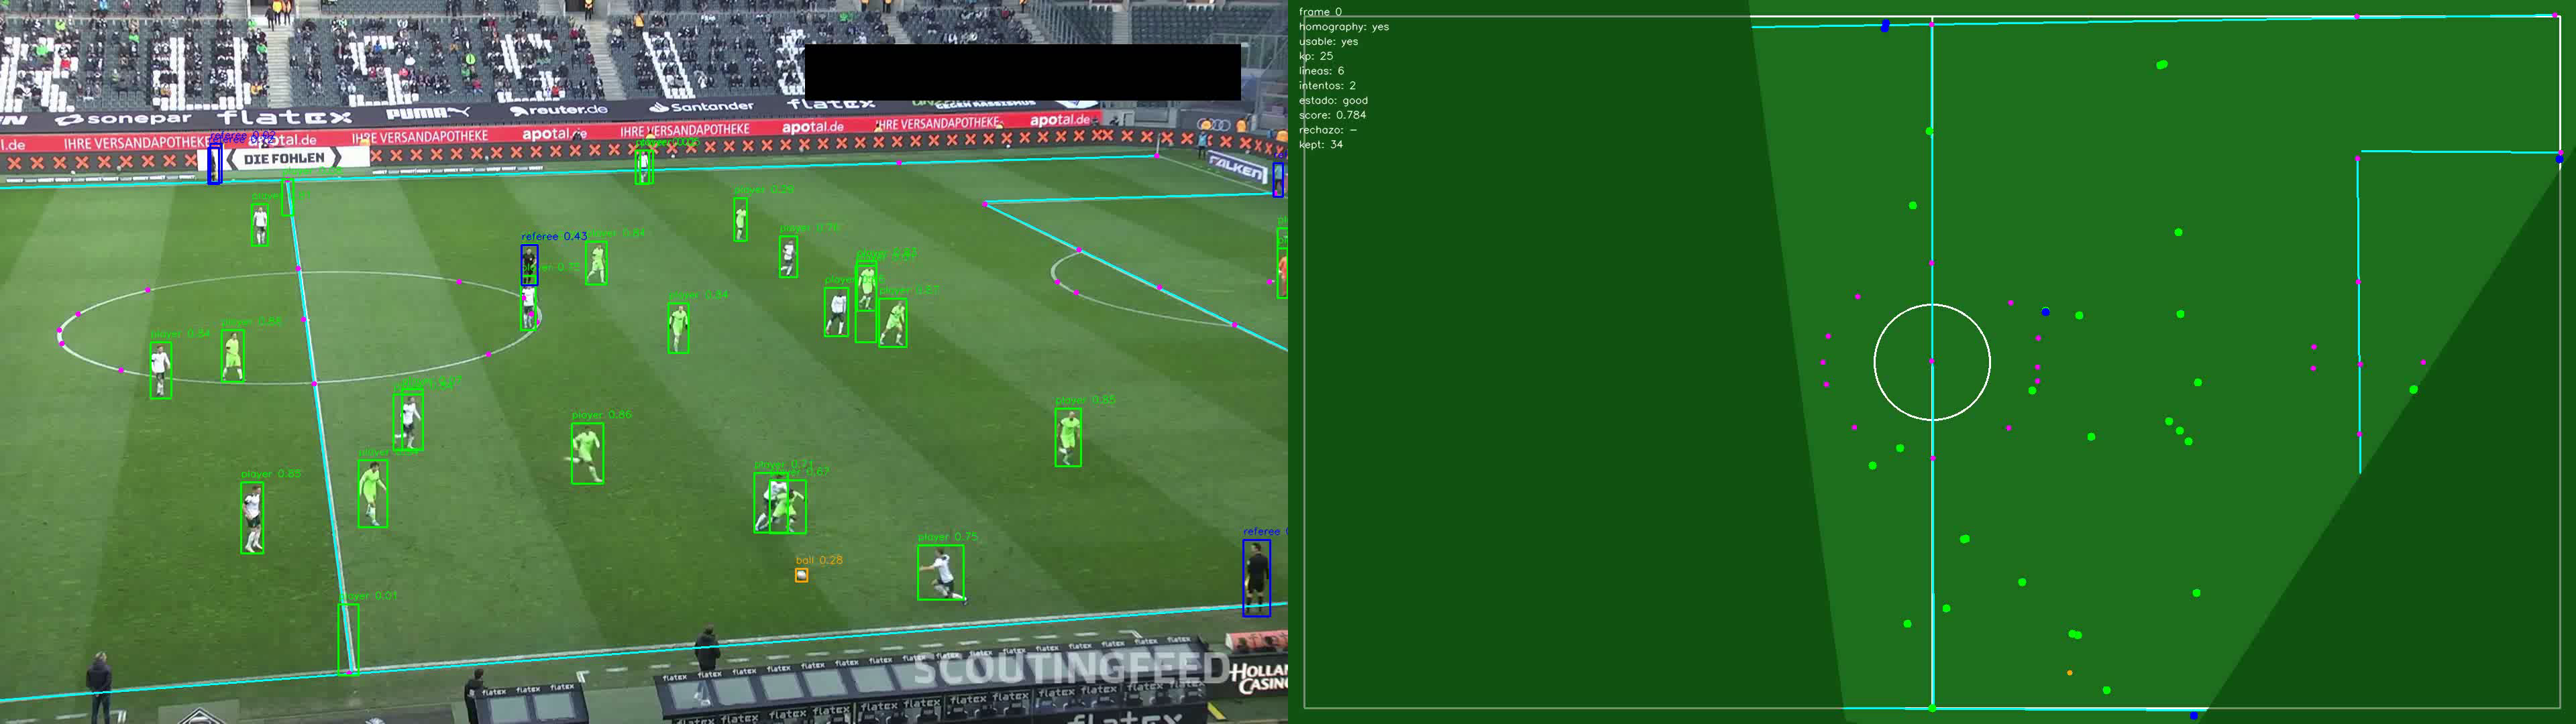
\includegraphics[width=0.85\textwidth]{Imagenes/Propias/homography_frame.png}
    \caption{Resultado visual de la fase de calibración del campo y proyección.}
    \label{fig:homography_frame}
\end{figure}

\section{Clasificación de equipos}

Tras la fase de calibración y proyección, el siguiente paso del pipeline consiste en identificar a qué equipo pertenece cada detección. El detector inicial permite diferenciar clases como jugador, portero, árbitro o balón, pero no proporciona directamente la pertenencia de equipo de cada futbolista. Para resolver esta limitación se implementa una fase específica de asignación basada en el color de la camiseta.

El planteamiento parte de una hipótesis sencilla: en un partido de fútbol, el rasgo visual más estable para distinguir a los jugadores de un equipo frente a los del rival es el color de la equipación. A partir de esta idea, la clasificación se divide en dos procesos: primero, la extracción del color representativo de la camiseta para cada detección candidata y después la asociación de ese color a uno de los dos equipos de campo presentes en el partido.

Todo este proceso se realiza en el espacio de color LAB. En este espacio, el canal $L$ representa la luminosidad, el canal $A$ codifica la oposición entre verde y rojo, y el canal $B$ codifica la oposición entre azul y amarillo. En la implementación de OpenCV estos valores se almacenan escalados en el rango $[0,255]$, con los canales $A$ y $B$ centrados aproximadamente en 128 para representar valores neutros. Se ha escogido LAB porque la distancia euclídea entre dos colores en este espacio se aproxima mejor a la diferencia perceptual que en RGB, lo que resulta útil para comparar colores de camisetas bajo distintas condiciones de iluminación. Aun así, este espacio no elimina por completo el efecto de sombras, reflejos o cambios de luz, especialmente porque el canal $L$ sigue dependiendo de la luminosidad de la imagen.

\subsection{Identificación del color de la camiseta}

La identificación del color de la camiseta parte de las cajas delimitadoras generadas por el detector. En la implementación se utilizan las coordenadas de la caja en formato $(x_1, y_1, x_2, y_2)$, que delimitan la región de la imagen donde se encuentra cada detección (jugador, portero o árbitro). Como la camiseta se encuentra normalmente en la parte superior del cuerpo, se recorta únicamente el 50\% superior del \textit{bounding box}. De esta forma se reduce la influencia del pantalón, las botas y parte del césped.

Esta aproximación no cubre todos los casos posibles. Por ejemplo, un jugador puede aparecer en el suelo, girado o parcialmente ocluido, pero estos casos son menos frecuentes y se asumen como excepciones dentro de un sistema que debe funcionar de forma robusta en la mayoría de frames.

Una vez extraída la región superior de la caja, todavía aparece un problema importante: el \textit{bounding box} es rectangular, mientras que el cuerpo del jugador no lo es. Por tanto, dentro del recorte no solo aparece la camiseta, sino también césped, cabeza, brazos u otros elementos de fondo. Para separar la camiseta del resto de píxeles se aplica KMeans con $k=2$ sobre los píxeles del recorte en espacio LAB. La idea es dividir los colores del recorte en dos grupos principales: uno correspondiente a la camiseta y otro correspondiente al fondo.

Aunque podrían plantearse más clusters, por ejemplo para separar cabeza, camiseta y césped, en la práctica $k=2$ ofrece un compromiso adecuado entre simplicidad, estabilidad y coste computacional. La cabeza o pequeñas regiones secundarias suelen quedar absorbidas por uno de los dos clusters, y su influencia sobre el centroide final es limitada si ocupan pocos píxeles frente a la camiseta o el fondo.

Para decidir qué cluster corresponde a la camiseta no se toma simplemente el cluster mayoritario, ya que en algunos recortes el fondo puede ocupar más superficie que el propio jugador. En su lugar, se selecciona un conjunto fijo de puntos de referencia del recorte (esquinas y bordes: superior-izquierda, superior-derecha, inferior-izquierda, inferior-derecha, centro superior, centro lateral izquierdo y centro lateral derecho). Estos puntos suelen pertenecer al fondo, por lo que el cluster más frecuente entre ellos se interpreta como fondo. El otro cluster se considera el de la camiseta, y su centroide LAB se guarda como color representativo de la detección.

\begin{equation}
\mathbf{c}_{\text{camiseta}} = [L, A, B]
\label{eq:color-camiseta-lab}
\end{equation}

Este proceso se aplica a cada detección (jugadores, árbitros y porteros). La decisión final de equipo y posibles reetiquetados de clase (por ejemplo, entre jugador, portero y árbitro) se realiza en la etapa de asociación descrita en el siguiente \hyperref[subsec:asociacionEquipo]{Apartado~\ref*{subsec:asociacionEquipo}}. En la \hyperref[fig:shirt-crop-kmeans]{Figura~\ref*{fig:shirt-crop-kmeans}} se muestra un ejemplo del recorte superior y la segmentación de color utilizada para estimar \(c_{camiseta}\).
\begin{figure}[H]
    \centering
    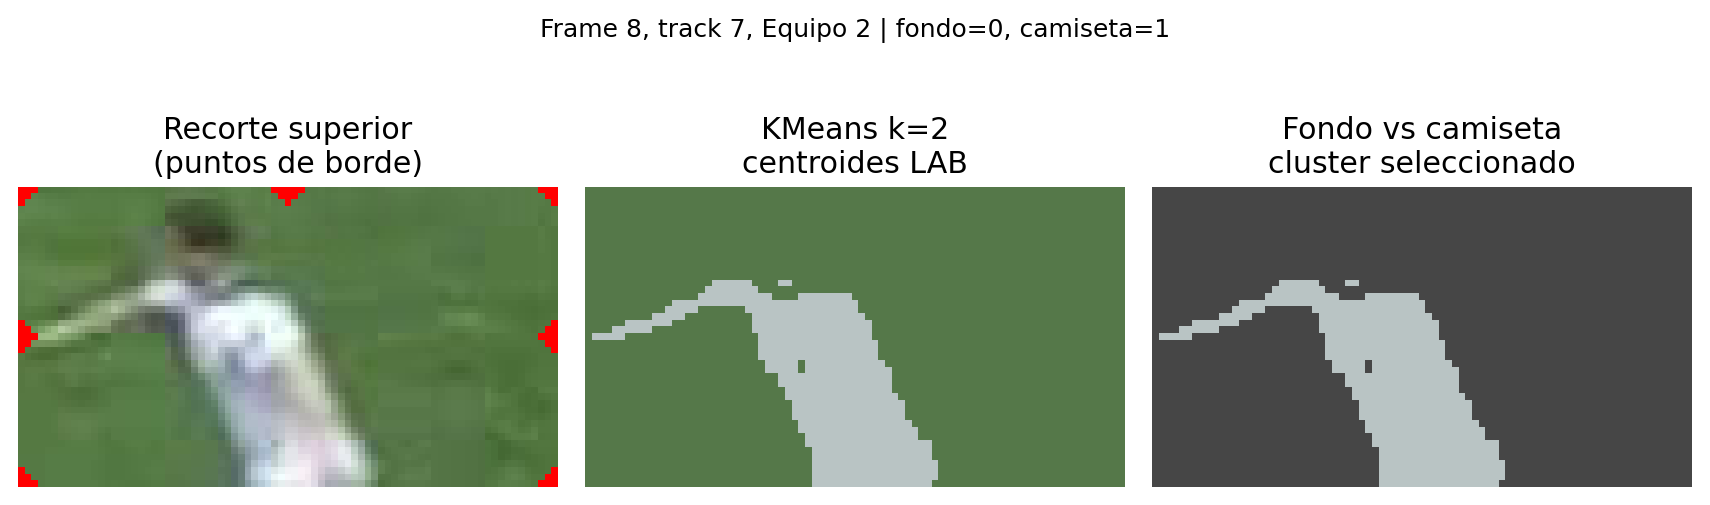
\includegraphics[width=0.9\textwidth]{Imagenes/Propias/shirt_crop_kmeans_example.png}
    \caption[Recorte de crop de jugador y KMeans]{Ejemplo de recorte superior de jugador y segmentación mediante KMeans con $k=2$.}
    \label{fig:shirt-crop-kmeans}
\end{figure}

\subsection{Asociación del equipo}
\label{subsec:asociacionEquipo}

En esta sección se describe la lógica para asociar cada track detectado a uno de los dos equipos.

\subsubsection{Asignación por color y centro del equipo}

Una vez obtenido el color de camiseta de cada detección candidata, representado por el vector $\mathbf{c}_{\text{camiseta}}$ definido en la Ecuación~\eqref{eq:color-camiseta-lab}, el objetivo es asociarlo a uno de los dos equipos de campo del partido. Para ello se acumulan muestras de colores LAB de las camistas de los jugadores y se aplica KMeans con $k=2$, esta vez no sobre píxeles individuales, sino sobre los colores de las camisetas ya extraídos. Cada cluster representa uno de los dos equipos de campo.

El centro de cada equipo se calcula mediante la mediana de las muestras LAB del cluster, en lugar de usar directamente la media. Esta decisión hace que la referencia de color sea más robusta frente a detecciones erróneas, sombras, reflejos o recortes en los que la camiseta no se haya aislado correctamente.

La asignación de una nueva detección se realiza calculando la distancia euclídea entre el color de su camiseta y el color de referencia de cada equipo:

\[
d(c, \mu_t) = \|c - \mu_t\|_2
\]

donde $c$ es el color LAB de la camiseta detectada y $\mu_t$ es el color representativo del equipo $t$. La detección se asigna al equipo cuya referencia esté más cerca:

\[
equipo(c) = \arg\min_t d(c, \mu_t)
\]


\subsubsection{Actualización online, \textit{bootstrap} y \textit{buckets} de muestras}

La construcción de clusters de color se realiza en modo online mediante un esquema de \textit{buckets} por clase, con dos contenedores principales: muestras de campo (\texttt{player}) y muestras de árbitro (\texttt{referee}). Cada nueva detección con color estimado solo se incorpora si supera una confianza mínima configurable.

Durante las primeras fases del vídeo, cuando los clusters de equipos todavía no están estabilizados, el sistema acumula muestras progresivamente y retrasa la actualización hasta disponer de soporte suficiente. Para el \textit{bucket} de jugadores, la actualización de centros no se lanza en cada frame, sino de forma periódica (cada 5 frames) y únicamente cuando se alcanza un mínimo de muestras acumuladas (en nuestra configuración, 60).

Cuando se ejecuta la actualización, se aplica KMeans con $k=2$ sobre las muestras LAB de jugadores. Después se valida el tamaño de los clusters obtenidos: si alguno resulta demasiado pequeño (por debajo de un mínimo configurable), se considera un cluster inválido, se descarta y se repite el ajuste sobre el cluster mayor. Si tras varias iteraciones no se obtiene una partición estable, la actualización se rechaza y se espera a nuevas muestras.

Además, para cada equipo se calculan estadísticas robustas de distancia intra-cluster (cuartiles e IQR), a partir de las cuales se define un umbral superior de pertenencia. Estas cotas se usan para detectar colores alejados del patrón esperado y limitar el impacto de \textit{outliers}.

En el caso del árbitro, el color de referencia no se estima con KMeans, sino mediante media recortada (\textit{trimmed mean}) sobre las muestras LAB acumuladas (recorte del 15\% por canal), lo que reduce la influencia de valores extremos y mejora la robustez del modelo.

En la \hyperref[fig:team-color-clusters-lab]{Figura~\ref*{fig:team-color-clusters-lab}} se puede ver como queda el estado de color de un partido después una ejecución. Se puede ver como el sistema es capaz de definir clusters bastante acertados sobre los colores de cada grupo de detecciones. Concretamente se puede ver el cluster del Equipo 1, de color verde, el cluster del Equipo 2, de color blanco, y el cluster de árbitros, de color negro. 

\begin{figure}[H]
    \centering
    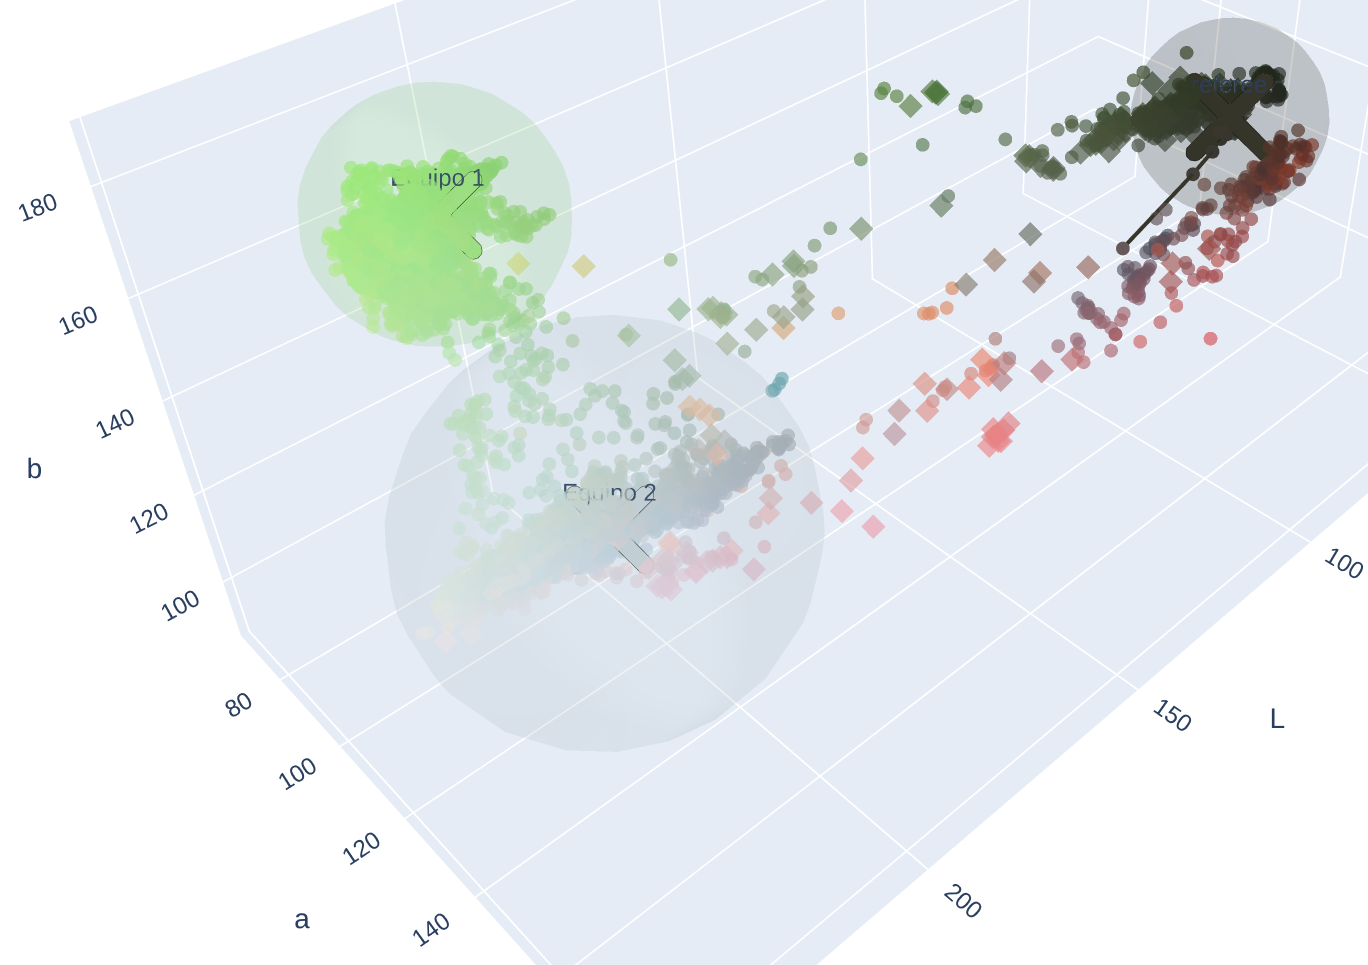
\includegraphics[width=0.7\textwidth]{Imagenes/Propias//lab_scatter_3d.png}
    \caption[Distribución de detecciones en el espacio LAB]{Distribución de detecciones en el espacio LAB, referencias de color y fronteras de pertenencia por equipo.}
    \label{fig:team-color-clusters-lab}
\end{figure}

\subsubsection{Reetiquetado de clase}

Una vez disponible el estado de color (centros de equipo, referencia de árbitro y umbrales de pertenencia), la inferencia por detección no se limita a asignar equipo: también puede reajustar la clase semántica final de la detección. En concreto, para cada candidato con color de camiseta estimado se calcula su distancia a los centros disponibles y, junto con restricciones posicionales en coordenadas de campo, se decide la etiqueta final entre \texttt{player}, \texttt{referee} y \texttt{goalkeeper}.

Si el color se asocia al patrón de árbitro, la detección solo se confirma como \texttt{referee} cuando también supera las compuertas posicionales definidas para ese rol (estar pegado a las líneas de banda o en una posición central del campo).

Cuando una detección queda fuera del patrón de equipos de campo pero su posición es compatible con portero, puede reetiquetarse como \texttt{goalkeeper}.

Para jugadores de campo, la pertenencia a equipo se valida además con umbrales robustos intra-cluster (derivados de cuartiles e IQR). Así, una detección no se acepta únicamente por vecino más cercano, sino también por consistencia estadística con el cluster de destino. 

En resumen, la salida de esta fase no es solo un color asignado a un equipo, sino una decisión conjunta \textit{clase + equipo} condicionada por evidencia cromática y geométrica, lo que mejora la robustez frente a confusiones entre jugador, árbitro y portero.

La \hyperref[fig:field-relabel-map]{Figura~\ref*{fig:field-relabel-map}} muestra el funcionamiento del re-etiquetado sobre coordenadas de campo. En naranja se representan los casos en los que una detección inicial de \texttt{player} se reclasifica como \texttt{referee}, y en azul los casos \texttt{player}$\rightarrow$\texttt{goalkeeper}. La distribución espacial de estos puntos coincide con lo que se observa en el vídeo de referencia: los re-etiquetados naranjas se concentran en la zona central, consistente con la trayectoria del árbitro principal, mientras que los re-etiquetados azules aparecen en el entorno del área izquierda, compatible con la posición típica de un portero. Además, los cambios se producen únicamente dentro de las regiones de validez definidas por las compuertas posicionales de cada clase.


\begin{figure}[H]
    \centering
    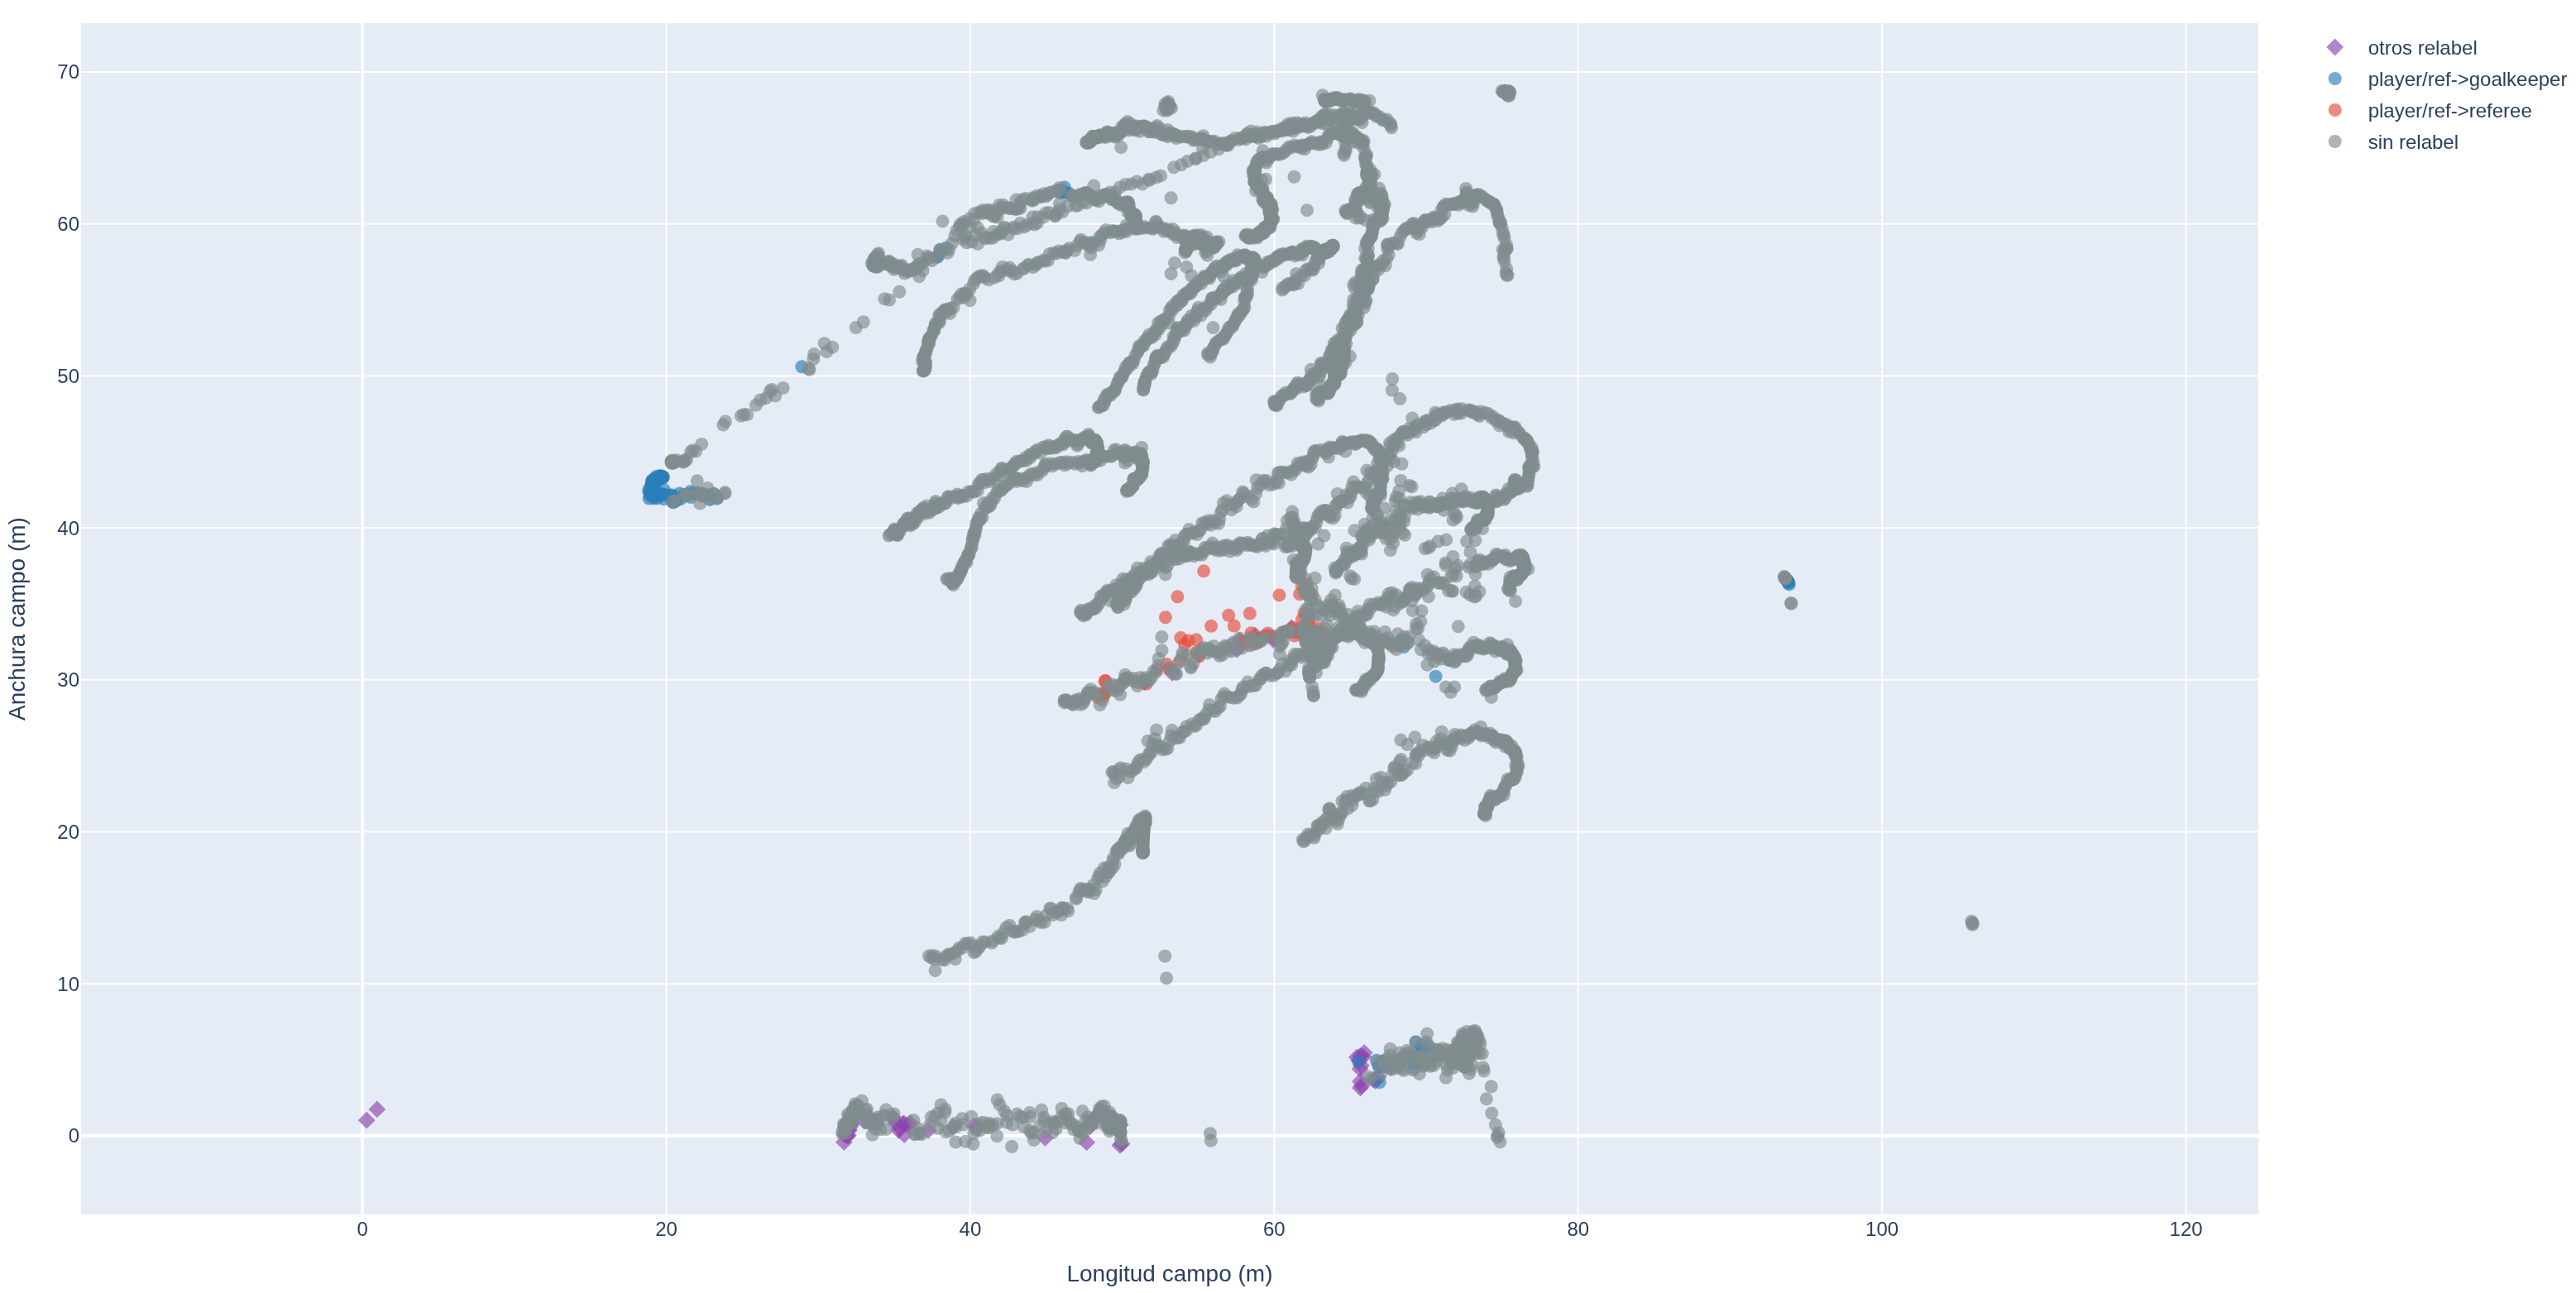
\includegraphics[width=0.95\textwidth]{Imagenes/Propias/field_relabel_map.png}
    \caption[Mapa de relabels en el campo]{Mapa de posiciones en campo con casos de relabel por categoría.}
    \label{fig:field-relabel-map}
\end{figure}


La configuración operativa del módulo se resume en la Tabla~\ref{tab:clasificacion_equipos}. 
\begin{table}[htbp]
    \centering
    \begin{tabular}{c|c}
        \textbf{Parámetro} & \textbf{Valor utilizado} \\
        \hline\hline
        Espacio de color & LAB \\
        Región analizada & 50\% superior del bounding box \\
        Clusters para camiseta & 2 \\
        Clusters para equipos de campo & 2 \\
        Muestras mínimas (\texttt{player}) & 60 acumuladas \\
        Muestras mínimas (\texttt{referee}) & 15 acumuladas \\
        Frecuencia de actualización de clusters & cada 5 frames \\
        Tamaño mínimo de cluster (\texttt{min\_size\_cluster}) & 15 \\
        Centro de equipo & mediana LAB del cluster \\
        Referencia de árbitro & \textit{trimmed mean} LAB (15\%) \\
        Distancia de asignación & euclídea en LAB \\
        \hline
    \end{tabular}
    \caption{Configuración principal del módulo de clasificación de equipos.}
    \label{tab:clasificacion_equipos}
\end{table}

Finalmente, cabe destacar que esta fase fue uno de los cuellos de botella iniciales del pipeline. En una primera versión, el clustering de cada camiseta se realizaba en CPU con \texttt{scikit-learn}, lo que incrementaba el tiempo de procesamiento por frame. Para reducir esta latencia se implementó una versión batched del KMeans con aceleración en GPU cuando está disponible (basada en \texttt{CuPy}), manteniendo \texttt{scikit-learn} como alternativa en CPU. En nuestras pruebas, esta optimización redujo el tiempo aproximado de identificación de camisetas y asignación de equipo de 1.5 s/frame a 0.05 s/frame, lo que supone una aceleración de aproximadamente $30\times$.


\section{Capa de asociacion temporal basada en ByteTrack}
\label{sec:bytetrack-layer}

El proceso de detección permite identificar que en un frame aparece un elemento de una determinada clase, pero cada frame se procesa de forma independiente. Para que el sistema pueda reconocer a un mismo jugador a lo largo del vídeo, no basta con detectar jugadores, porteros, árbitros y balón en cada imagen: es necesario asociar las detecciones de frames consecutivos y mantener una identidad temporal estable. Este proceso se conoce como \textit{tracking multiobjeto}.

En nuestro caso, el tracking es una fase crítica porque gran parte de la información posterior depende del identificador asignado a cada elemento. Si un jugador recibe un ID distinto cada vez que aparece, no es posible construir su trayectoria, asociarle una posición, vincularlo a una alineación o utilizarlo correctamente en la generación de eventos. Por ello, el objetivo no es únicamente dibujar bounding boxes sobre el vídeo, sino mantener una representación persistente del partido. Idealmente, la salida final debe estar limitada a los elementos reales del juego: 20 jugadores de campo, 2 porteros, 3 árbitros y 1 balón.

Esta fase ha sido una de las más complejas del proyecto. En fútbol aparecen muchos problemas propios del dominio: oclusiones entre jugadores, cruces continuos, jugadores del mismo equipo con apariencia muy parecida, cambios de escala por el zoom, movimientos de cámara, detecciones perdidas durante varios frames y elementos que salen temporalmente del plano. Además, intentar solucionar uno de estos problemas de forma aislada puede empeorar otro. Por ejemplo, permitir reasociaciones muy amplias ayuda a recuperar jugadores tras una oclusión, pero también aumenta el riesgo de intercambiar IDs entre jugadores cercanos. Por ello, el sistema se ha construido como una combinación de varias restricciones complementarias.

La fase de asociacion temporal se ha dividido en dos capas. La primera capa, tratada en esta seccion, es una adaptacion de ByteTrack orientada a producir asociaciones robustas entre detecciones consecutivas. La segunda capa, descrita en la \hyperref[sec:tracking-canonico]{Seccion~\ref*{sec:tracking-canonico}}, intenta coser esas asociaciones de ByteTrack para estabilizar las 26 identidades finales del partido.

En la \hyperref[sec:tracking-tecnologias]{Seccion~\ref*{sec:tracking-tecnologias}} se introdujo ByteTrack desde un punto de vista general. En este apartado se describe su integracion concreta como primera capa de tracking del pipeline visual y las modificaciones realizadas sobre el algoritmo clásico.

\subsection{Base de la fase}

Sobre la estructura original de ByteTrack se han añadido señales propias del proyecto: clase reajustada, equipo estimado y posicion proyectada sobre el campo.

La fase consume las detecciones enriquecidas de identificacion y produce una salida intermedia de detecciones asociadas con \textit{raw tracker id}. Esta salida no es todavia la identidad final del jugador, sino una asociacion temporal que alimentará la siguiente capa.

\subsection{Asociacion multi-etapa en cada frame}

Manteniendo la logica general explicada en la \hyperref[sec:tracking-tecnologias]{Figura~\ref*{sec:tracking-tecnologias}}, la implementacion actual ejecuta seis subfases de matching en vez de las 3 descritas en \hyperref[sec:tracking-tecnologias]{2.4}:
Manteniendo la logica general de ByteTrack descrita en la \hyperref[sec:tracking-tecnologias]{Sección~\ref*{sec:tracking-tecnologias}} (asociacion progresiva de tracks activos, perdidos y no confirmados), nuestra adaptación desdobla el matching en seis subfases, ampliando el esquema base presentado en 2.4.
\begin{itemize}
    \item \texttt{high\_iou}
    \item \texttt{low\_iou}
    \item \texttt{unconfirmed\_iou}
    \item \texttt{high\_bbox}
    \item \texttt{low\_bbox}
    \item \texttt{unconfirmed\_bbox}
\end{itemize}

Mientras que las primeras tres subfases usan el solape entre cajas como función de coste, las últimas 3 subfases, utilizan la distancias entre los centros de las \textit{bounding box}, y actuan como rescate cuando el solape no es suficiente, reduciendo fragmentaciones en escenas con zoom, paneos y discontinuidades de deteccion.

\subsection{Restricciones por clase y equipo}

Otra mejora introducida sobre ByteTrack consiste en utilizar la clase del objeto y el equipo asignado como restricciones de asociación. Si un ID canónico corresponde a un jugador, no debería poder reasociarse con una detección de balón o de árbitro. Del mismo modo, si un jugador pertenece a un equipo, no debería heredar la identidad de un jugador del equipo contrario.

Por lo tanto, en nuestra adaptación del ByteTrack, se usan la clase de la detección y su equipo asociado como restricciones de asociación duras. Si la clase del track y la clase de la deteccion candidata no coinciden, la asociacion se descarta automáticamente.

Del mismo modo, para \texttt{player}, cuando hay informacion de equipo tanto en el track como en la detección, se aplica también una restricción dura: si no coinciden, la asociacion se descarta.

Estas restricciones reducen los intercambios entre elementos de distinta clase y entre jugadores de equipos diferentes. Sin embargo, todavía puede haber intercambios entre jugadores del mismo equipo, especialmente cuando se cruzan o aparecen muy juntos en la imagen. Para reducir este problema fue necesario incorporar información geométrica del campo.

\subsection{Uso de homografia y restricción espacial en metros}

En nuestra versión de ByteTrack adaptada también se aplica un gate espacial en campo para las clases \texttt{player} y \texttt{goalkeeper}. Si la distancia proyectada entre el track y la detección candidata supera el límite configurado (8 metros), la asociación se descarta. En cambio, si está dentro del rango permitido, la pareja se mantiene como factible y el coste se decide por el criterio de matching de la subfase (IoU o distancia de centros en las fases de rescate).

Durante el desarrollo se evaluó usar la posición de las detecciones proyectada al campo como coste principal de la asociación. En la practica, esta opción degradaba el rendimiento ya que esta señal presentaba mucha vibracion frame a frame debido a pequeños cambios en la homografía entre frames.  Por este motivo había variaciones bruscas en las trayectorias estimadas de las identidades. Esto afectaba especialmente a la prediccion del estado con el filtro de Kalman y acababa propagando errores al proceso de matching. Por este motivo, en la version final la posicion en campo se utiliza como compuerta geometrica de factibilidad (gate duro) y no como termino principal de coste.

\subsection{Control de creacion de nuevos tracks}

Otro problema relevante es la creacion excesiva de nuevos tracks. Esto puede ocurrir cuando el detector produce bounding boxes duplicados o cuando ByteTrack pierde temporalmente una identidad. Para reducir este efecto, se añadieron reglas de supresión por solape de tracks nuevos:
\begin{itemize}
    \item contra tracks activos ya consolidados,
    \item contra tracks tentativos no confirmados,
    \item y entre candidatos nuevos del mismo frame.
\end{itemize}

Un candidato a track nuevo se descarta si solapa demasiado con un track activo, si solapa con un track tentativo no consolidado, o si solapa con otro candidato nuevo de mayor confianza. Ante cualquier solape entre dos candidatos nuevos, se conserva únicamente el de mayor confianza. Con esta regla se consigue reducir tracks duplicados sin alterar el seguimiento de tracks ya consolidados.

La configuración concreta de estos umbrales de solape se resume en la \hyperref[tab:supresion-nuevos-tracks-bytetrack]{Tabla~\ref*{tab:supresion-nuevos-tracks-bytetrack}}.

\begin{table}[htbp]
    \centering
    \scriptsize
    \begin{tabular}{c|c|p{7.5cm}}
        \textbf{Concepto} & \textbf{Valor} & \textbf{Funcion} \\
        \hline\hline
        Solape maximo con tracks activos & 0.2 & Evita crear un nuevo ID sobre un track ya consolidado. \\
        Solape maximo con tracks tentativos & 0.1 & Evita duplicados sobre tracks aun no consolidados. \\
        Solape entre candidatos nuevos & 0.0 & Conserva solo el candidato nuevo de mayor confianza si hay solape. \\
        \hline
    \end{tabular}
    \caption{Reglas de supresion en la creacion de nuevos tracks de ByteTrack.}
    \label{tab:supresion-nuevos-tracks-bytetrack}
\end{table}

\subsection{Resumen de la capa}

En resumen, esta fase no se limita a ejecutar ByteTrack sobre cajas de YOLO, sino que integra restricciones de clase, equipo, geometria en campo y control de creación de tracks para mejorar la asociacion temporal en video de futbol broadcast. La capa siguiente toma estas asociaciones y construye las identidades canonicas estables del partido.

\section{Capa de tracking canónico}
\label{sec:tracking-canonico}

La salida de la capa de asociación basada en ByteTrack (Seccion~\ref{sec:bytetrack-layer}) proporciona asociaciones robustas entre detecciones consecutivas de frames cercanos, pero esos IDs internos no garantizan por sí solos estabilidad global durante todo el partido. Cuando hay oclusiones largas, salidas de plano o cambios de escala bruscos, un mismo jugador puede reaparecer con otro \textit{tracker id}.

Por este motivo, el pipeline incorpora una segunda capa: la canonización. Su objetivo es transformar las asociaciones \textit{raw} en identidades finales estables, con límites por clase y reglas específicas para jugadores, porteros, árbitros y balón.

De esta forma, podría ocurrir que, por ejemplo, un jugador esté asociado al \textit{tracker id} 14 durante una parte del vídeo, se pierda durante varios frames y reaparezca con \textit{tracker id} 37. Si la capa canónica determina que ambos tracks corresponden al mismo jugador, entonces se conservará el mismo \textit{id canónico} para los dos tramos.

\subsection{Entrada de la capa y objetivo de canonización}

La capa canónica consume el paquete devuelto por la capa de ByteTrack y opera sobre detecciones ya asociadas, junto con metadatos de clase, equipo, posición en el campo y confianza. A partir de esa entrada, decide para cada detección si:
\begin{itemize}
    \item mantiene continuidad con un ID canonico existente,
    \item reengancha un ID canonico previo sobre un nuevo \textit{raw tracker id},
    \item crea una identidad canonica nueva dentro de los limites permitidos,
    \item o descarta la deteccion si no cumple los criterios de consistencia.
\end{itemize}

\subsection{Proceso de asignación canónica por frame}

En cada frame, la capa canónica aplica un flujo secuencial compacto. Primero intenta mantener continuidad directa entre \textit{raw tracker ids} ya conocidos y sus IDs canónicos previos, siempre que la compatibilidad de clase/equipo y las compuertas de continuidad sean válidas según la \hyperref[subsec:continuidad-canonica-reasignacion]{Subseccion~\ref*{subsec:continuidad-canonica-reasignacion}} y la \hyperref[subsec:reasignacion-sin-homografia]{Subseccion~\ref*{subsec:reasignacion-sin-homografia}}.

Despues, con los tracks de ByteTrack que no han sido resueltos en esa primera fase, se abre una fase de reasignación sobre IDs canónicos perdidos o libres, respetando de nuevo las reglas de continuidad en campo y en imagen definidas en la \hyperref[subsec:continuidad-canonica-reasignacion]{Subseccion~\ref*{subsec:continuidad-canonica-reasignacion}} y la \hyperref[subsec:reasignacion-sin-homografia]{Subseccion~\ref*{subsec:reasignacion-sin-homografia}}.
Si un track de ByteTrack sigue sin una asignación válida, la capa evalúa la creación de un nuevo slot canónico dentro de los límites y reservas definidos en la \hyperref[tab:limites-canonicos]{Tabla~\ref*{tab:limites-canonicos}} y explicados en la \hyperref[subsec:ids-canonicos-limites]{Subseccion~\ref*{subsec:ids-canonicos-limites}}.

Sobre ese flujo base se aplican reglas específicas por clase, detalladas en sus apartados correspondientes: porteros en la \hyperref[subsec:tratamiento-porteros]{Subseccion~\ref*{subsec:tratamiento-porteros}}, árbitros en la \hyperref[subsec:tratamiento-arbitros]{Subseccion~\ref*{subsec:tratamiento-arbitros}}, balón en la \hyperref[subsec:seguimiento-balon-canonico]{Subseccion~\ref*{subsec:seguimiento-balon-canonico}} y reabsorción conservadora en la \hyperref[subsec:reabsorcion-identidades]{Subseccion~\ref*{subsec:reabsorcion-identidades}}.

\subsection{IDs canónicos y límites por clase}
\label{subsec:ids-canonicos-limites}

A diferencia de ByteTrack, que puede crear tracks internos adicionales de forma flexible, la capa canónica impone una estructura final acotada.

En la configuración actual, los slots canónicos quedan reservados de forma explicita: el balón se fija en el ID 0, los porteros ocupan los IDs 1 y 2, los jugadores de campo se reparten en dos bloques por equipo (3--12 y 13--22), y, por último, los arbitros usan los IDs 23, 24 y 25. Además, los slots de árbitro no son intercambiables: 23 se asocia al arbitro central, 24 al asistente de la banda superior y 25 al asistente de la banda inferior. La \hyperref[tab:limites-canonicos]{Tabla~\ref*{tab:limites-canonicos}} resume esta asignación junto con los limites finales por clase.

\begin{table}[htbp]
    \centering
    \scriptsize
    \begin{tabular}{c|c|p{7.5cm}}
        \textbf{Parametro} & \textbf{Valor} & \textbf{Descripcion} \\
        \hline\hline
        \texttt{max\_tracks\_per\_class.player} & 20 & Jugadores de campo en slots canonicos de equipo (3--12 y 13--22). \\
        \texttt{max\_tracks\_per\_class.goalkeeper} & 2 & Porteros con IDs reservados (1 y 2). \\
        \texttt{max\_tracks\_per\_class.referee} & 3 & Arbitro central y asistentes con IDs reservados (23, 24, 25). \\
        \texttt{max\_tracks\_per\_class.ball} & 1 & Balon, almacenado siempre con ID 0. \\
        \hline
    \end{tabular}
    \caption{Limites de identidades canonicas por clase y asignacion de slots.}
    \label{tab:limites-canonicos}
\end{table}


\subsection{Continuidad canonica y reasignacion}
\label{subsec:continuidad-canonica-reasignacion}

Cuando hay posicion proyectada fiable en campo, la continuidad de \texttt{player}/\texttt{goalkeeper} se valida con un gate metrico dependiente de los frames perdidos. El gate parte de un valor base y crece de forma controlada hasta un maximo, evitando saltos fisicamente incompatibles y permitiendo recuperar identidades tras oclusiones cortas.

Siendo \(f\) el numero de frames desde la ultima observacion valida del ID canonico. El gate se calcula con base \(g_0=2.1\) m, decaimiento \(\delta=0.3\) m/frame, tope temporal \(f_{\max}=10\) y cap absoluto \(G_{\max}=8.0\) m:

\[
f'=\min(f,f_{\max}),
\qquad
G(f)=\min\!\left(
G_{\max},
\sum_{i=0}^{f'-1}\max(g_0-\delta i,0)
\right).
\]

Con los valores usados en el proyecto:

\[
G(1)=2.1,\;
G(2)=3.9,\;
G(3)=5.4,\;
G(4)=6.6,\;
G(5)=7.5,\;
G(6)=8.0,
\]

y a partir de ahi queda saturado en \(8.0\) m. Una candidata en campo se considera factible solo si su distancia al estado canonico cumple:

\[
d_{\text{campo}} \leq G(f).
\]

\subsection{Reasignación cuando no hay homografía fiable}
\label{subsec:reasignacion-sin-homografia}

Cuando no hay homografía válida, la capa canónica utiliza la posición en imagen como respaldo. En ese caso, no puede medir distancias en metros, por lo que utiliza el centro de la bounding box y el histórico de movimiento del track.

Si todavía no hay suficiente histórico, se permite únicamente una tolerancia mínima de 10 píxeles. Cuando el track ya tiene al menos 3 muestras de movimiento, se calcula el desplazamiento medio por frame, $\overline{d}$, y se estima cuánto podría haberse movido durante los frames perdidos:

\[
D_{esperado} =
\overline{d} \cdot \min(f,12) \cdot 0.75
\]

donde $f$ es el número de frames perdidos. El valor 12 actúa como límite máximo de extrapolación: aunque un jugador lleve perdido más frames, el radio de búsqueda no sigue creciendo indefinidamente. El factor 0.75 hace que esta estimación sea conservadora, evitando abrir demasiado el radio de búsqueda. La \hyperref[tab:movimiento-imagen]{Tabla~\ref*{tab:movimiento-imagen}} resume los valores de los hiperparámetros.

\begin{table}[htbp]
    \centering
    \scriptsize
    \begin{tabular}{c|c|p{7.5cm}}
        \textbf{Parametro} & \textbf{Valor} & \textbf{Funcion} \\
        \hline\hline
        \texttt{reassign\_min\_distance} & 10 px & Radio minimo cuando todavia no hay historico suficiente. \\
        \texttt{reassign\_motion\_growth\_cap\_frames} & 12 & Limita el numero de frames durante los que el radio de busqueda puede crecer. \\
        \texttt{reassign\_min\_samples} & 3 & Observaciones necesarias para estimar el desplazamiento medio. \\
        \texttt{reassign\_motion\_factor} & 0.75 & Reduce la distancia extrapolada para evitar reasociaciones demasiado amplias. \\
        \hline
    \end{tabular}
    \caption{Restricciones de movimiento usadas cuando no hay homografía fiable.}
    \label{tab:movimiento-imagen}
\end{table}

\subsection{Tratamiento específico de porteros}
\label{subsec:tratamiento-porteros}

Los porteros presentan un problema particular: en muchos planos tácticos o de inicio de jugada no aparecen en cámara. Si el sistema esperase únicamente a detectarlos, podrían recibir IDs tardíos o inestables. Para evitarlo, se crean dos identidades canónicas reservadas en los puntos de penalti del campo. Estas identidades se corresponden con los IDs 1 y 2.

Estas detecciones no proceden de YOLO, sino que son semillas sintéticas generadas a partir de la geometría del campo. Mientras no haya una detección real compatible, se almacenan con confianza 0 y sin equipo asignado. Cuando aparece una detección de clase \textit{goalkeeper} compatible, la capa canónica asigna ese track sintético a la detección compatible.

El radio de absorción desde el punto de penalti es de 20 metros. Aunque parece un valor alto, no significa que cualquier jugador pueda absorber el ID del portero. Primero, solo se consideran detecciones compatibles con la clase \texttt{goalkeeper}. Segundo, la semilla está situada en el punto de penalti, pero el portero real puede aparecer sobre la línea de gol, dentro del área pequeña, desplazado lateralmente o con error de homografía. Por eso se utiliza un radio amplio, protegido por la restricción de clase. La \hyperref[tab:seeds-porteros]{Tabla~\ref*{tab:seeds-porteros}} resume los hiperparametros de configuracion asociados a estas semillas canónicas de portero.

\begin{table}[htbp]
    \centering
    \scriptsize
    \begin{tabular}{c|c|p{7.5cm}}
        \textbf{Concepto} & \textbf{Valor} & \textbf{Función} \\
        \hline\hline
        \texttt{reserve\_penalty\_spot\_seed\_match\_distance\_m} & 20 m & Fija el radio maximo de absorcion entre una seed de portero y una deteccion real compatible. \\
        \hline
    \end{tabular}
    \caption{Configuración de identidades sintéticas reservadas para porteros.}
    \label{tab:seeds-porteros}
\end{table}

\subsection{Tratamiento específico de árbitros}
\label{subsec:tratamiento-arbitros}

También se reservan IDs específicos para los árbitros. En concreto, el ID 23 se asocia al árbitro central, el 24 al árbitro asistente de la parte superior de la imagen y el 25 a su homólogo de la parte inferior. Esto se hace para no tratarlos como tres árbitros intercambiables y, así, evitar intercambios entre ellos.

Las detecciones de clase árbitro se asocian a uno de los tracks canónicos de árbitro de banda si su posición proyectada está a menos de 3 metros de la línea lateral.

Para el ID 23 asociado al árbitro central, se añade una restricción horizontal calculada a partir de los jugadores y porteros visibles. En cada frame se recogen las coordenadas $(x, y)$ proyectadas al campo de todas las detecciones y se ordenan por su coordenada $x$. Si existen al menos 4 posiciones válidas, se define como rango permitido el intervalo entre la segunda posición más a la izquierda y la segunda posición más a la derecha. De esta forma, una detección muy extrema en el campo no puede absorber el ID del árbitro central. Si no hay suficientes jugadores proyectados, esta restricción horizontal no se aplica.

\subsection{Reabsorción de identidades perdidas}
\label{subsec:reabsorcion-identidades}

Debido a las reglas de continuidad anteriores, puede ocurrir que un jugador desaparezca durante un tramo largo y vuelva con un \textit{raw tracker id} nuevo. Si todos los IDs canónicos ya están creados, se han alcanzado los límites por clase definidos en la \hyperref[tab:limites-canonicos]{Tabla~\ref*{tab:limites-canonicos}} y ningún track canónico compatible está lo suficientemente cerca del raw track de ByteTrack como para absorberlo, entonces ese track se quedará perdido en el limbo sin materializarse como track canónico real y se perderá esa identidad. Para estos casos, la capa canónica incorpora una reabsorción forzada orientada a recuperar estos tracks perdidos de la forma más segura posible.

El mecanismo se activa solo para \texttt{player}. Primero se identifican IDs canónicos de jugador que llevan perdidos al menos 20 frames. En paralelo, se buscan tracks \textit{raw} huérfanos que no hayan sido asignados en el frame actual y que se hayan mantenido al menos 10 frames consecutivos con clase \texttt{player} y el mismo equipo.

Con esos candidatos, la capa construye emparejamientos posibles únicamente dentro del mismo equipo. Cuando hay varios candidatos compatibles, se prioriza la asociación con mayor consistencia espacial y temporal (menor distancia respecto al último estado canónico útil), de modo que el track huérfano más compatible se reenganche al ID canónico perdido.

De este modo, la reabsorción actúa como una vía de recuperación tardía, pero con condiciones estrictas de clase, equipo y consistencia espacial.

\subsection{Seguimiento del balón}
\label{subsec:seguimiento-balon-canonico}

El balón se gestiona de forma distinta a los jugadores. Es un objeto más pequeño, con menor confianza de detección y movimientos más bruscos. Por ello, además de las detecciones devueltas por ByteTrack, se conservan candidatas crudas de YOLO con una confianza mínima muy baja, y la capa canónica selecciona una única candidata por frame.

Si el balón ya había sido visto recientemente, se estima una posición esperada a partir de su movimiento inmediato anterior (desplazamiento entre las últimas observaciones válidas) y se proyecta esa tendencia sobre los frames perdidos. Con esa predicción se aplica un gate posicional dinámico: parte de un radio base de 90 píxeles y crece con los frames perdidos (35 píxeles por frame). En paralelo, también se comprueba la compatibilidad de tamaño para descartar cambios de escala no plausibles.

Cuando una candidata tiene confianza alta (\(\geq 0.6\)), las restricciones se relajan de forma controlada: tanto el radio posicional como el ratio de tamaño permitido se escalan por 1.4. Todas estas restricciones y configuraciones se reflejan en la \hyperref[tab:balon-tracking]{Tabla~\ref*{tab:balon-tracking}}.

Si ninguna candidata resulta coherente con la predicción temporal y las validaciones de tamaño, el sistema prefiere dejar el frame sin balón antes que aceptar una detección errónea. El balón se almacena siempre con ID canónico 0.

\begin{table}[htbp]
    \centering
    \scriptsize
    \begin{tabular}{c|c|p{7.5cm}}
        \textbf{Concepto} & \textbf{Valor} & \textbf{Función} \\
        \hline\hline
        \texttt{ball\_min\_conf} & 0.0035 & Permite considerar candidatas debiles antes del filtrado temporal. \\
        \texttt{ball\_expected\_position\_gate\_px} & 90 px & Define el radio base alrededor de la posicion esperada del balon. \\
        \texttt{ball\_expected\_position\_gate\_growth\_per\_frame} & 35 px & Amplia el gate posicional por cada frame perdido. \\
        \texttt{ball\_expected\_position\_confidence\_relax} & 1.4 & Relaja el gate posicional y el ratio de tamano cuando la candidata tiene alta confianza. \\
        \texttt{ball\_size\_ratio\_per\_frame} & 1.8 & Limita los cambios de escala plausibles entre observaciones consecutivas. \\
        \texttt{ball\_size\_min\_samples} & 5 & Numero minimo de observaciones para activar la comprobacion estadistica de tamano. \\
        \texttt{ball\_size\_std\_factor} & 3.0 & Factor multiplicativo usado en la banda estadistica de tamano aceptable. \\
        \texttt{ball\_size\_std\_floor} & 1.0 & Impone un suelo para que la banda estadistica de tamano no colapse. \\
        \texttt{ball\_max\_reassign\_lost\_frames} & 30 & Limita la ventana tras la que deja de intentarse continuidad con el ultimo estado valido del balon. \\
        \texttt{ball\_high\_conf\_override} & 0.6 & Define el umbral a partir del cual una candidata se trata como deteccion de alta confianza. \\
        \hline
    \end{tabular}
    \caption{Restricciones temporales utilizadas para seleccionar el balón.}
    \label{tab:balon-tracking}
\end{table}

La configuracion de esta capa se resume en la \hyperref[tab:hiperparametros-canonico]{Tabla~\ref*{tab:hiperparametros-canonico}}. Esta tabla final solo recoge los parametros del bloque de track \texttt{canonical} que no se han detallado ya en tablas especificas anteriores de esta misma seccion.

\begin{table}[htbp]
\centering
\scriptsize
\setlength{\tabcolsep}{3pt}
\renewcommand{\arraystretch}{1.12}
\begin{tabularx}{\textwidth}{
>{\raggedright\arraybackslash}p{2.6cm}
>{\raggedright\arraybackslash}p{3.4cm}
>{\raggedright\arraybackslash}p{1.5cm}
>{\raggedright\arraybackslash}X
}
\toprule
\textbf{Bloque} & \textbf{Parámetro} & \textbf{Valor} & \textbf{Uso en pipeline} \\
\midrule

Continuidad en campo &
\texttt{field\_gate\_m} &
\texttt{2.1} &
Controla la distancia máxima permitida para reasignar tracks usando posición proyectada al campo. \\

&
\texttt{field\_max\_lost} &
\texttt{10} &
Limita el número de frames perdidos durante los que se permite recuperar una identidad mediante continuidad en campo. \\

&
\texttt{field\_gate\_cap\_m} &
\texttt{8.0} &
Acota el radio máximo de búsqueda en coordenadas métricas. \\

&
\texttt{field\_decay} &
\texttt{0.3} &
Reduce progresivamente la tolerancia de reasignación a medida que el track lleva más tiempo perdido. \\

\midrule

Reglas de árbitro &
\texttt{ref\_sideline\_band\_m} &
\texttt{3.0} &
Restringe los slots de árbitro de banda y ayuda a evitar intercambios entre árbitros. \\

\midrule

Reabsorción forzada &
\texttt{forced\_abs\_min\_lost} &
\texttt{20} &
Permite recuperar de forma tardía tracks huérfanos de jugadores solo tras un número mínimo de frames perdidos. \\

&
\texttt{forced\_abs\_min\_consist} &
\texttt{10} &
Exige consistencia temporal antes de reabsorber un raw track en una identidad canónica. \\

\bottomrule
\end{tabularx}

\caption[Hiperparámetros de la capa de tracking canónico]{
Hiperparámetros principales de la capa de tracking canónico.}
\label{tab:hiperparametros-canonico}
\end{table}

El valor final de los parámetros se describe en la \hyperref[sec:evaluacion-heuristica-depuracion]{Seccion~\ref*{sec:evaluacion-heuristica-depuracion}}.

\subsection{Salida del tracking}

La salida final del tracking se almacena como una estructura organizada por clase y por frame. Para cada elemento se guarda su bounding box, confianza, equipo asignado, color de camiseta, tamaño de la bounding box, ID interno de ByteTrack, ID canónico y posición proyectada al campo.

Esta información resulta fundamental para las fases posteriores del proyecto, ya que permite construir trayectorias, analizar estabilidad temporal, generar métricas y transformar los datos al formato requerido por los módulos de análisis de eventos.

En resumen, el tracking implementado combina detección, equipo, clase, homografía, restricciones geométricas, control de movimiento, límites por clase, IDs canónicos y reglas particulares para porteros, árbitros y balón. Esta combinación es necesaria para reducir pérdidas de identidad e intercambios entre jugadores en un escenario especialmente complejo como el vídeo broadcast de fútbol.

\section{Evaluacion heuristica y depuracion del pipeline visual}
\label{sec:evaluacion-heuristica-depuracion}

\subsection{Ausencia de \textit{ground truth} anotado}

Durante el desarrollo no se dispuso de un conjunto de datos anotado frame a frame que pudiera usarse como \textit{ground truth} para evaluar de forma supervisada todo el pipeline de procesamiento visual. Por ese motivo, la validacion del sistema se apoyo en una estrategia heuristica, combinando inspeccion visual y metricas agregadas tras cada ejecucion.

En particular, la inspeccion cualitativa se realizo sobre un video de prueba de referencia\footnote{\url{https://github.com/hectorgarciaa/narrador-futbol/blob/main/data/partidoPrueba/partido.mp4}}, revisando la evolucion temporal de las identidades y la consistencia de los tracks en situaciones dificiles (oclusiones, cruces, perdidas temporales y reapariciones).

\subsection{Metricas heuristicas principales}

Tras ejecutar el tracking, el sistema calcula un resumen de metricas para jugadores y balon. Entre ellas se incluyen la cobertura media, que mide durante que proporcion del video aparece cada ID; el numero medio de fragmentos, que indica cuantas interrupciones tiene una trayectoria; la longitud media de los huecos sin deteccion; la velocidad media y maxima estimada a partir del movimiento de las \textit{bounding boxes}; la tasa de cambios de equipo asignado; la entropia del equipo, que refleja la inestabilidad en la asignacion; la variacion del color de camiseta; la variacion del tamano de la \textit{bounding box}; y la confianza media de las detecciones asociadas a cada track.

\subsection{Uso de metricas para ajuste de hiperparametros}

Estas metricas fueron especialmente utiles para guiar la depuracion de todos los modulos visuales y no solo del tracking canonico. Por ejemplo, velocidades maximas excesivamente altas solian indicar intercambios de identidad entre jugadores lejanos; una cobertura baja podia senalar perdidas frecuentes de deteccion o \textit{gates} demasiado estrictos; y un numero alto de fragmentos apuntaba a trayectorias poco continuas.

Del mismo modo, cambios frecuentes de equipo o una alta variacion del color de camiseta podian revelar errores de clasificacion o reasignacion. Por tanto, la evaluacion del pipeline visual se apoyo en dos fuentes complementarias: inspeccion visual del video generado y analisis cuantitativo de metricas. La primera permitia entender el tipo de error y su contexto, mientras que la segunda permitia comparar ejecuciones y verificar si una modificacion mejoraba realmente la estabilidad global del sistema.




\textbf{IMAGEN DE 4 ID BYTETRACK ID CANONICOS ID FINALES Y BIRD EYE SIN POSICIONES}